\documentclass[
	% -- opções da classe memoir --
	12pt,				% tamanho da fonte
	openright,			% capítulos começam em pág ímpar (insere página vazia caso preciso)
	oneside,			% para impressão em frente e verso. Oposto a oneside
	a4paper,			% tamanho do papel.
	% -- opções da classe abntex2 --
	chapter=TITLE,		% títulos de capítulos convertidos em letras maiúsculas
	%section=TITLE,		% títulos de seções convertidos em letras maiúsculas
	%subsection=TITLE,	% títulos de subseções convertidos em letras maiúsculas
	%subsubsection=TITLE,% títulos de subsubseções convertidos em letras maiúsculas
	% -- opções do pacote babel --
	english,			% idioma adicional para hifenização
	french,				% idioma adicional para hifenização
	spanish,			% idioma adicional para hifenização
	brazil				% o último idioma é o principal do documento
	]{abntex2}

% ---
% Pacotes básicos 
% ---
\usepackage{lmodern}			% Usa a fonte Latin Modern
\usepackage{mathptmx}			% Usa a fonte Times New Roman
\usepackage[T1]{fontenc}		% Selecao de codigos de fonte.
\usepackage[utf8]{inputenc}		% Codificacao do documento (conversão automática dos acentos)
\usepackage{lastpage}			% Usado pela Ficha catalográfica
\usepackage{indentfirst}		% Indenta o primeiro parágrafo de cada seção.
\usepackage{color}				% Controle das cores
\usepackage{graphicx}			% Inclusão de gráficos
\usepackage{subcaption}				% Inclusão de gráficos lado a lado
\usepackage{microtype} 			% para melhorias de justificação
\usepackage{tabularx,ragged2e}	% Para inserir tabelas
\usepackage{multirow}			% Para mesclar células
\usepackage[dvipsnames,table,xcdraw]{xcolor}		% Permite adicionar cores nas linhas de tabelas
\usepackage{fancyvrb}			% Permite adicionar arquivos de texto
\usepackage[portuguese, ruled, linesnumbered]{algorithm2e} % Uso de algoritmos
\usepackage{amsfonts}			% Permite usar notação de conjuntos
\usepackage{amsmath}			% Permite citar equações
\usepackage{amsthm}				% Permite criar teoremas e experimentos
\usepackage{amssymb}            % Usei para o símbolo de transposto
\usepackage[font={bf, small}, labelsep=endash, labelfont=bf]{caption}	% Faz legenda de figuras ficarem em negrito
\usepackage[final]{pdfpages}
\usepackage{textcomp}           % para não dar erro no gensymb
\usepackage{gensymb}            % Para inserir o símbolo de grau em ângulos
\usepackage{enumitem}           % Para criar listas "numeradas" por letras (no abntex2 tem alineas no lugar)
\usepackage{bm,amsbsy}          % Para usar símbolos em negrito

\newcolumntype{L}{>{\RaggedRight\arraybackslash}X}
% ---

\usepackage[alf, abnt-emphasize=bf]{abntex2cite}	% Citações padrão ABNT
\usepackage{modelo-ufpa/ufpa}

% Muda o título de lista de ilustrações para lista de figuras
\addto\captionsbrazil{%
  \renewcommand{\listfigurename}%
    {Lista de Ilustrações}%
	\renewcommand{\listtablename}%
    {Lista de Tabelas}%
}

% Permite utilizar figuras sem precisar colocar o caminho absoluto
\graphicspath{{imagens/}}

% Define o ambiente de experimentos
\theoremstyle{definition}
\newtheorem{experimento}{Experimento}[section]
\newcommand{\experimentoautorefname}{Experimento}

%% Novo estilo
\makepagestyle{estilo_pretextual} %%% escolha um nome
  \makeevenhead{estilo_pretextual}{}{}{\ABNTEXfontereduzida \textbf \thepage}
  \makeoddhead{estilo_pretextual}{}{}{\ABNTEXfontereduzida \textbf \thepage}

%% Customiza comando \pretextual
\renewcommand{\pretextual}{
  \pagenumbering{roman} %%% ou \pagenumbering{Roman}
  \aliaspagestyle{chapter}{estilo_pretextual}% customizing chapter pagestyle
  \pagestyle{estilo_pretextual}
  \aliaspagestyle{cleared}{empty}
  \aliaspagestyle{part}{estilo_pretextual}
}

% ---
% Ajusta a marca \textual para que a numeração volte a ser arábica
% nos elementos textuais
\let\oldtextual\textual        % copia o comando \textual anterior para \oldtextual
\renewcommand{\textual}{%
  \oldtextual%
  \pagenumbering{arabic} % volta à numeração arábica
}
% ---


% ---
% Informações de dados para CAPA, FOLHA DE ROSTO e FICHA CATALOGRÁFICA
% ---
\universidade{Universidade Federal do Pará}
\instituto{Instituto de Tecnologia}
\faculdade{Programa de Pós-Graduação em Engenharia Elétrica}
\titulo{Nome do trabalho}
\autor{Weverson Vieira do Nascimento}
\local{Belém - PA}
\data{\the\year}
\tipotrabalho{Dissertação}
\grau{Mestre em Engenharia Elétrica } % manter o espaço no final
\preambulo{Dissertação apresentada como exigência parcial para obtenção do grau de \imprimirgrau pela \imprimiruniversidade. Área de concentração: Engenharias.}
\sobrenome{Nascimento}
\nome{Weverson Vieira do}
\palavraschave{
primeira.
segunda.
terceira.
quarta.
quinta.
}

% orientadores
\orientador{Prof. Dr. Fulano}
%\coorientador{Prof. Dr. Ciclano}
\datadadefesa{Data da Defesa: \underline{\qquad \qquad\qquad}}% janeiro de 2018}
\conceito{Conceito: \underline{\qquad\qquad\qquad}}
\primeiromembrodabanca{Prof.ª Dra. Ciclana}
\segundomembrodabanca{Prof. Dr. Fulano}
%\terceiromembrodabanca{Prof. Dr. Nome Sobrenome}
%\quartomembrodabanca{Prof. Dr. Outro Nome}
\faculdadecoordenador{Prof.ª Dra. Maria Emília de Lima Tostes}
% ---
% informações do PDF
\makeatletter
\hypersetup{
     	%pagebackref=true,
		pdftitle={\imprimirtitulo}, 
		pdfauthor={\imprimirautor},
    	pdfsubject={\imprimirpreambulo},
	    pdfcreator={LaTeX with abnTeX2},
		pdfkeywords={\imprimirpalavraschave}, 
		colorlinks=true,       		% false: boxed links; true: colored links
    	linkcolor=black,          	% color of internal links
    	citecolor=black,        		% color of links to bibliography
    	filecolor=magenta,      		% color of file links
		urlcolor=black,
		bookmarksdepth=4,
        breaklinks=true
}
\makeatother
% --- 

% --- 
% Espaçamentos entre linhas e parágrafos 
% --- 

% O tamanho do parágrafo é dado por:
\setlength{\parindent}{1.3cm}

% Controle do espaçamento entre um parágrafo e outro:
\setlength{\parskip}{0.2cm}  % tente também \onelineskip
\linespread{1.5} % espaçamento entre linhas

% ---
% compila o indice
% ---
\makeindex
% ---


% ----
% Início do documento
% ----
\begin{document}
\selectlanguage{brazil}
\frenchspacing 

% ----------------------------------------------------------
% ELEMENTOS PRÉ-TEXTUAIS
% ----------------------------------------------------------
% \pretextual

% ---
% Capa (obrigatório)
% ---
\imprimircapa
% ---

% ---
% Folha de rosto (obrigatório)
% ---
\imprimirfolhaderosto
% ---
% a ficha catalográfica oficial é a gerada pela biblioteca da instituição
% deve constar na versão final
% na ausência, usar a gerada pelo modelo
% \begin{fichacatalografica}
%     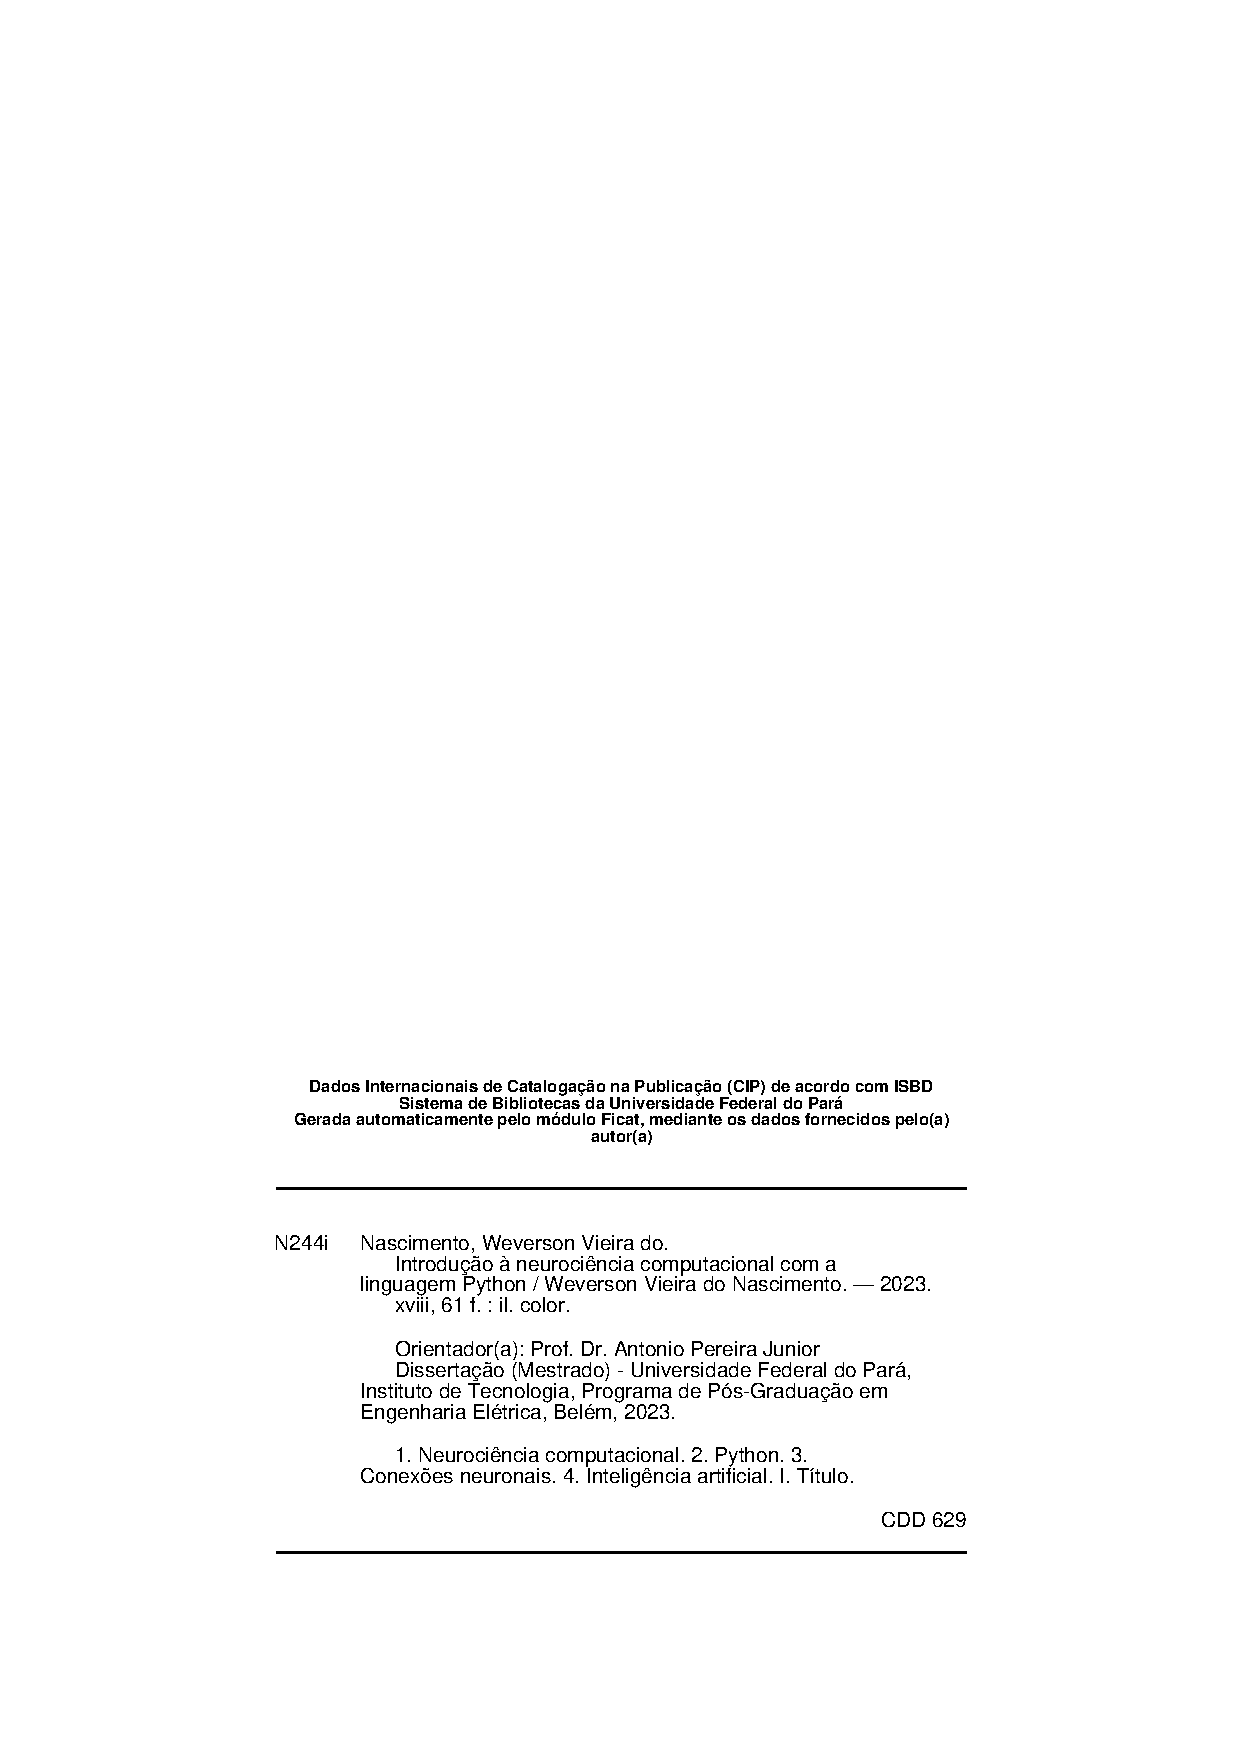
\includepdf{modelo-ufpa/ficha.pdf}
% \end{fichacatalografica}
\newpage
\begin{fichacatalografica}
	\imprimirfichacatalografica
\end{fichacatalografica}

% ---
% Inserir folha de aprovação (obrigatório)
% ---
% na versão final deve-se incluir a folha assinada
% \includepdf{folhadeaprovacao_final.pdf}
\begin{folhadeaprovacao}
	\ufpaPaginaDeAprovacao
    %\imprimirfolhadeaprovacao
\end{folhadeaprovacao}
% ---

% ---
% Dedicatória (opcional)
% ---
\begin{dedicatoria}
   \vspace*{\fill}
   \noindent
   \begin{flushright}
      \textit{escreva}\\
      \textit{aqui}\\
      \textit{a}\\
      \textit{dedicatória}
   \end{flushright}
\end{dedicatoria}
% ---

% ---
% Agradecimentos (opcional)
% ---
\begin{agradecimentos}
a escrever.
\end{agradecimentos}
% ---

% ---
% Epígrafe (opcional - NBR 10520)
% ---
\begin{epigrafe}
    \vspace*{\fill}
	\begin{flushright}
		\textit{``texto da epígrafe''\\
		autor}
	\end{flushright}
\end{epigrafe}
% ---

% ---
% RESUMOS
% ---
\setlength{\absparsep}{18pt}
\begin{resumo}
%O  resumo  deve  ressaltar  o  objetivo,  o  método,  os  resultados  e  as  conclusões  do  documento.  A  ordem  e  a  extensão destes itens dependem do tipo de resumo (informativo ou indicativo) e do tratamento que cada item recebe no documento original.
%O  resumo  deve  ser  composto  de  uma  sequência  de  frases  concisas,  afirmativas  e  não  de  enumeração  de  tópicos. Recomenda-se o uso de parágrafo único.
%A  primeira  frase  deve  ser  significativa,  explicando  o  tema  principal  do  documento.  A  seguir,  deve-se  indicar  a informação sobre a categoria do tratamento (memória, estudo de caso, análise da situação etc.).
texto do resumo

\textbf{Palavras-chave}: \imprimirpalavraschave
\end{resumo}

\begin{resumo}[Abstract]
 \begin{otherlanguage*}{english}
abstract

   \vspace{\onelineskip}
 
   \noindent 
   \textbf{Keywords}: escrever manualmente.
 \end{otherlanguage*}
\end{resumo}

% ---
% inserir lista de ilustrações (opcional)
% ---
\pdfbookmark[0]{\listfigurename}{lof}
\listoffigures*
\cleardoublepage
% ---

% ---
% inserir lista de quadros (não existe na norma, consta como ilustração)
% ---
%\pdfbookmark[0]{\listofquadrosname}{loq}
%\listofquadros*
%\cleardoublepage
% ---

% ---
% inserir lista de tabelas (opcional)
% ---
\pdfbookmark[0]{\listtablename}{lot}
\listoftables*
\cleardoublepage
% ---

% ---
% inserir lista de algoritmos (não consta na norma)
% ---
%\pdfbookmark[0]{\listalgorithmcfname}{loa}
%\imprimirlistadealgoritmos
%\cleardoublepage
% ---

% ---
% inserir lista de abreviaturas e siglas (opcional)
% ---
% listar em ordem alfabética
\begin{siglas}
\item[UFPA] Universidade Federal do Pará
\end{siglas}
% ---

% ---
% inserir lista de símbolos (opcional)
% ---
% inserir na ordem que aparecem no texto
\begin{simbolos}
\item[$\alpha$] Estrela de maior brilho de uma constelação % eu gosto de ver estrelas (literalmente)
\end{simbolos}
% ---

% ---
% inserir o sumario (obrigatório - NBR 6027)
% ---
\pdfbookmark[0]{\contentsname}{toc}
\tableofcontents*
\cleardoublepage
% ---

% ----------------------------------------------------------
% ELEMENTOS TEXTUAIS
% ----------------------------------------------------------
\textual

\chapter{Introdução}\label{cap:introducao}
\section{Contexto}

\section{Justificativa}

\section{Objetivos}
\subsection{Objetivo Geral}
Elaborar um roteiro para execução de um curso introdutório em neurociências computacionais usando linguagens de programação livres

\subsection{Objetivos Específicos}
\begin{itemize}
\item Obter uma bibliografia robusta para servir de base na elaboração do roteiro
\item Criar um conjunto de códigos contendo exemplos dos conceitos apresentados ao longo do roteiro
\item Consolidar o material criado em uma estrutura de fácil uso por interessados no tema em questão
\end{itemize}

\section{Metodologia}

\section{Estrutura do Trabalho}
O trabalho está estruturado da seguinte maneira: o Capítulo~\ref{cap:teoria} mostra os elementos da base teórica apresentada. Uma breve apresentação de definições sobre fisiologia, equações diferenciais ordinárias, probabilidade, noções sobre algoritmos e linguagem de programação são mostradas. O Capítulo~\ref{cap:temas} contém os temas teóricos e práticos que constituem o roteiro em si. O Capítulo~\ref{cap:conclusoes} contém as conclusões acerca do trabalho e os desdobramentos possíveis para este.

\chapter{Base teórica}\label{cap:teoria}
\section{Introdução}\label{sec:teoria_intro}
Dada a variedade de estudantes que podem ingressar em um curso de neurociência computacional, muitos deles podem não ter tido algumas disciplinas de base que são necessárias para um bom entendimento do conteúdo apresentado. Por isso, este capítulo contém uma base teórica útil para um nivelamento dos estudantes das mais diversas áreas. As sessões seguintes contemplam conteúdos de neurobiologia, equações diferenciais ordinárias, probabilidade e algoritmos.

\section{Neurobiologia básica}\label{sec:fisiologia}
O neurônio é a unidade básica do sistema nervoso. É composto pelo corpo celular (chamado de soma), dendritos, que recebem sinais de outros neurônios, axônio, que transmite os sinais a serem recebidos por outros neurônios, e terminais axônicos, que são as extremidades do axônio e se conectam com os dendritos de outros neurônios. Como outras células do corpo humano, o neurônio é composto por íons e moléculas, ambas podendo possuir cargas positivas ou negativas. A célula neuronal é revestida por uma bi-camada lipídica, e geralmente o interior dela possui uma maior concentração de cargas negativas, fazendo com que o potencial de membrana ($V_m$), que é a diferença de potencial entre a parte interna e a externa da célula neuronal ($V_M=V_{dentro}-V_{fora}$), fique a maior parte do tempo com valor negativo. O potencial de membrana se altera quando há o fluxo de íons através dos poros de canais iônicos (Figura~\ref{fig:membrananeuronio}).

\begin{figure}[tb]
	\centering
	\caption[Membrana do neurônio]{Membrana do neurônio}
	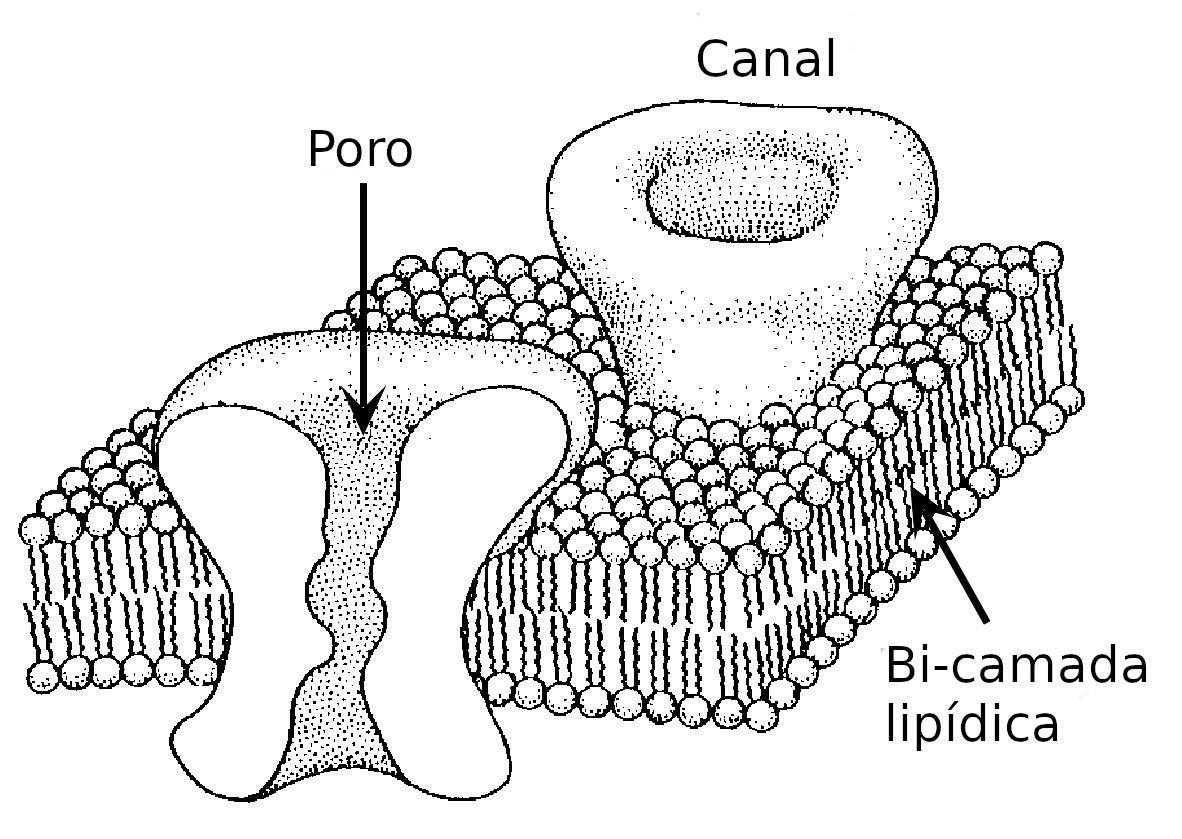
\includegraphics[width=0.55\linewidth]{figs/membrana_neuronio}
	\label{fig:membrananeuronio}
	\\
	Fonte: adaptado de \cite{hille_ionic_1992}
	%% adaptado de hille 1992 (pág. 170 pdf)
\end{figure}

Os canais iônicos são canais proteicos na membrana da célula neuronal e permitem a movimentação de íons através deles, como mostrado na Figura~\ref{fig:canaisions}. Podem ser de dois tipos: com ou sem portão. Canais sem portão estão sempre abertos, enquanto os com portão podem abrir ou fechar, dependendo do valor do potencial de membrana, e por isso são chamados de canais iônicos dependentes de tensão. Quando o fluxo de corrente elétrica de todos os íons é equilibrado dentro e fora da célula neuronal (ou seja, o potencial de membrana não se altera), ele é chamado de potencial de repouso (ou de equilíbrio). O valor típico é próximo de $-70\ mV$. O valor do potencial de repouso é calculado com base na concentração de cada íon dentro e fora da célula neuronal usando a equação de Nernst, dada por:
$$
E_A=\frac{k_BT}{z_Aq_e}ln\Big(\frac{A_{fora}}{A_{dentro}}\Big)
$$
sendo $A$ o íon, $z_A$ a carga do íon, $A_{fora}$ e $A_{dentro}$ a concentração desse íon fora e dentro da célula neuronal, respectivamente, $T$ a temperatura absoluta (em Kelvin), $k_B$ a a constante de \textit{Boltzmann} ($1,39*10^{-23}\ JK^{-1}$) e $q_e$ a carga elétrica fundamental ($1,6*10^{-19}\ C$). Os valores de cargas, concentração e potencial de Nernst para alguns íons são apresentados na Tabela~\ref{tab:concentracao_nernst}.

\begin{figure}[tb!]
	\centering
	\caption[Canais iônicos de potássio]{Canais iônicos de potássio. Em \textbf{a} os íons de potássio saem da célula, causando um excesso de cargas positivas fora e negativas dentro. Em \textbf{b} o fluxo para fora e dentro é igual, causando equilíbrio}
	\label{fig:canaisions}
	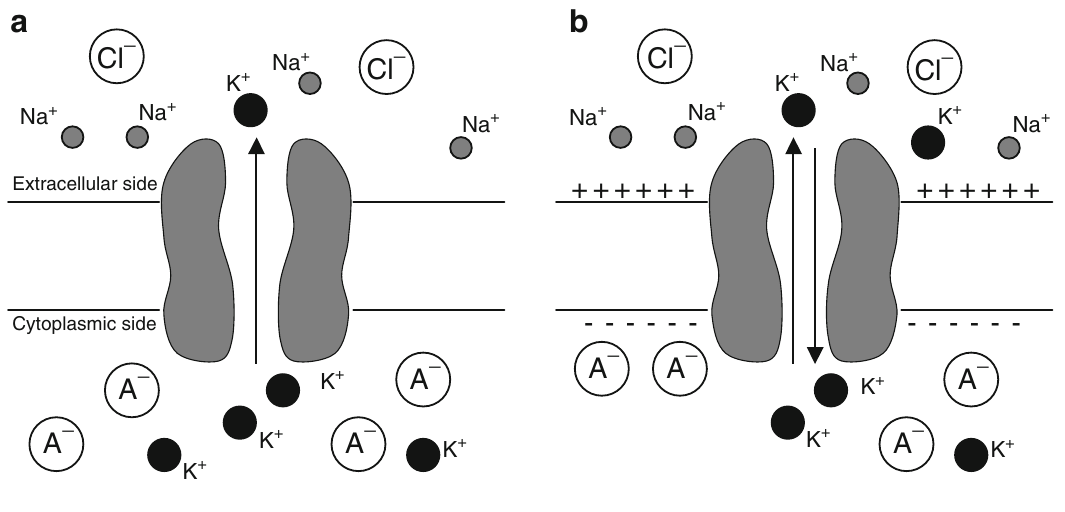
\includegraphics[width=0.7\linewidth]{figs/canais_ions}
	\\
	\cite{ermentrout_mathematical_2010}
\end{figure}

\begin{table}
	\centering
	\caption[Concentração de íons]{Concentração de íons}
	\label{tab:concentracao_nernst}
	\begin{tabular}{c|c|c|c|c}
		\hline
		Íon & Carga & Conc. interna ($nM$) & Conc. externa ($nM$) & Potencial de reversão ($mV$) \\
		\hline
		Sódio & +1 & 15 & 120 & 61,6 \\
		\hline
		Potássio & +1 & 150 & 6 & -86,1 \\
		\hline
		Cloreto & -1 & 52 & 560 & -65 \\
		\hline
		Cálcio & +2 & 50 & 2 & 141,7 \\
		\hline
	\end{tabular}
\end{table}

Fora do repouso, a diferença de potencial entre o interior e o exterior do neurônio produz movimentação iônica. Quando íons positivos (como $Na^+$ ou $Ca^{2+})$ entram na célula neuronal, o potencial de membrana fica menos positivo (até próximo de 0 mV), fenômeno conhecido como despolarização. De maneira semelhante, quando íons negativos (como $K^+$) saem da célula neuronal, ou negativos (como $Cl^-$) entram, o potencial de membrana fica mais negativo, fenômeno conhecido como hiperpolarização. Devido ao excesso de cargas negativas no interior da célula neuronal, e a existência de cargas positivas no exterior, a membrana do neurônio acaba funcionando como um capacitor, criando uma capacitância ($C_m$). O fluxo de íons através de canais sem portão é considerado constante, podendo ser agrupado em um elemento chamado de vazamento (\textit{leak}, em inglês), possuindo um potencial ($E_l$) e uma condutância ($G_l$), que é a facilidade desse elemento permitir o fluxo de corrente (o inverso da resistência). Com isso, é possível escrever uma equação relacionando o potencial de membrana da célula neuronal e os elementos de vazamento, como segue:
$$
\frac{\mathrm{d}V_m}{\mathrm{d}t}=G_l(E_l-V_m)/C_m
$$
que é dada na forma de uma equação diferencial, detalhada na seção seguinte.

\section{Equações diferenciais ordinárias}\label{sec:eqdif}
\begin{itemize}
	\item Equação diferencial ordinária: uma equação relacionando uma função desconhecida $y(t)$, algumas derivadas de $y(t)$ e a variável $t$, geralmente representando o tempo \cite{adkins_ordinary_2012}
	\item Ordem: a ordem da maior derivada que aparece na equação diferencial
	\item $t$: variável independente
	\item $y$: variável dependente (depende de $t$)
	\item A solução é uma família de equações, que depende da escolha de constantes
\end{itemize}

\begin{figure}[htb!]
	\centering
	\caption{Soluções $y(t) = t + 1 + ce^t$ da equação $y'=y-t$ para vários $c$}
	\label{fig:solucao}
	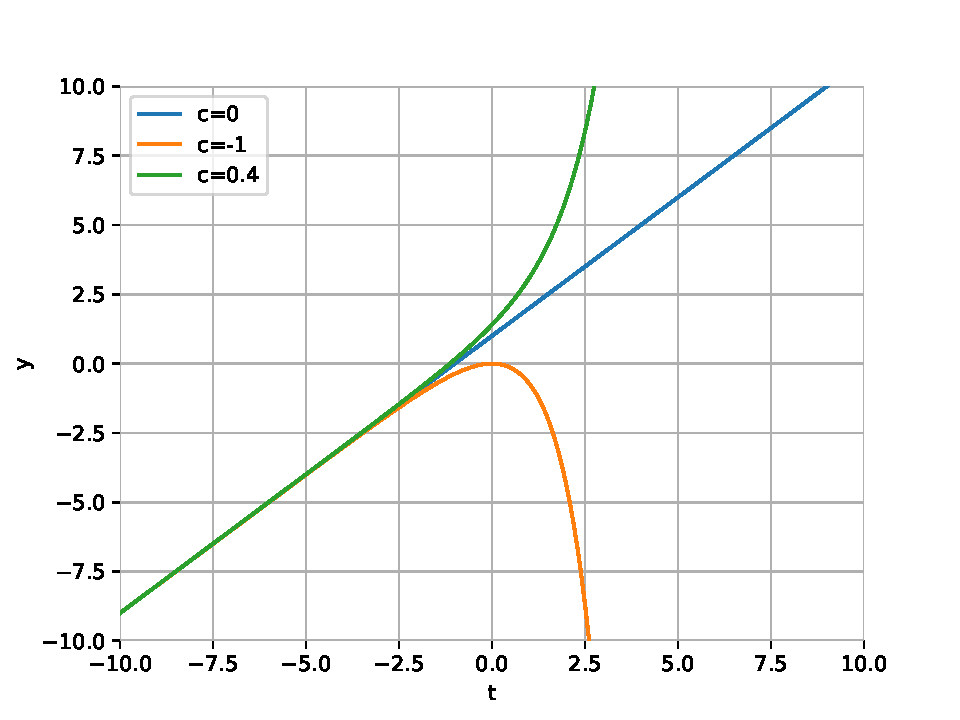
\includegraphics[width=0.7\linewidth]{figs/solucao}
\end{figure}


\subsection{Exemplos}
\subsubsection{Decaimento radioativo}
Segundo a lei do decaimento radioativo, a taxa na qual os átomos radioativos desintegram é proporcional ao número total de átomos radioativos presente. Sendo $N(t)$ o número de átomos radioativos no tempo $t$, então $N'(t)$ é a taxa de mudança. A lei do decaimento radioativo é a que segue:

$$N'(t) = -\lambda N(t)$$
onde $\lambda$ é a constante de decaimento.

\begin{figure}[htb!]
	\centering
	\caption{Decaimento radioativo ($\lambda = 0,5$)}
	\label{fig:decaimento}
	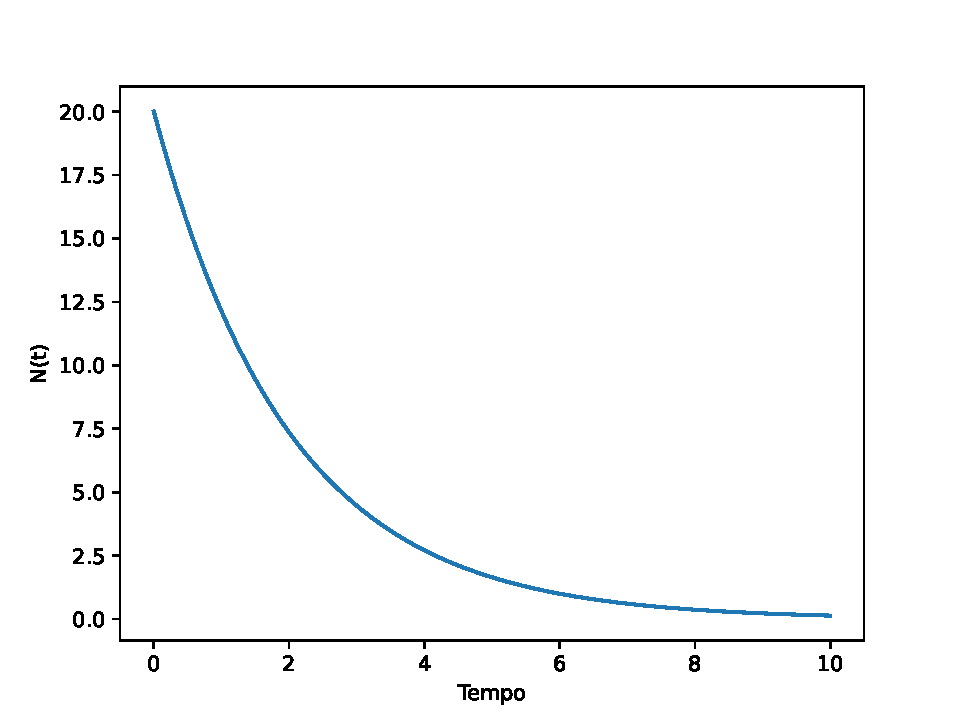
\includegraphics[width=0.7\linewidth]{figs/decaimento}
\end{figure}

\subsubsection{Equações de Lotka-volterra}
Também conhecidas como equações predador-presa, são um par de equações diferenciais de primeira ordem, frequentemente usadas para descrever a dinâmica de sistemas biológicos de interação entre duas espécies, uma como predadora e a outra como presa. As populações de cada uma das espécies são dadas pelo par de equações:

$$
x' = ax - bxy
$$$$
y' = dxy - cy
$$
onde:\\
$
x: \text{população da presa}\\
y: \text{população do predador}\\
x', y': \text{taxas de variação de cada população}\\
a, b, c, d: \text{parâmetros que descrevem a interação entre as espécies}
$

\begin{figure}[htb!]
	\centering
	\caption{Sistema de Lotka-Volterra ($a$ = 1,5; $b$ = 1; $c$ = 3; $d$ = 1)}
	\label{fig:lotka-volterra}
	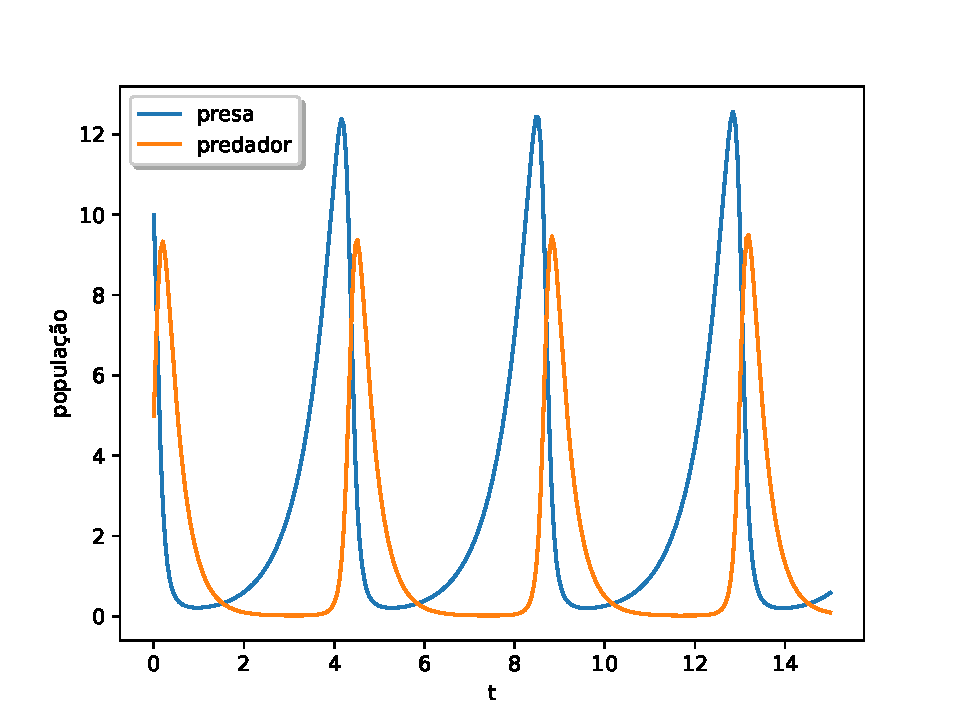
\includegraphics[width=0.7\linewidth]{figs/lotka-volterra}
\end{figure}


\subsubsection{Trajetória pendular}
O pêndulo é um dispositivo que contém uma massa atrelada a um fio e que oscila em torno de um ponto fixo. A equação do movimento para o ângulo $\theta$ (o ângulo que o pêndulo faz com a vertical) é:

$$
\frac{d^2\theta}{dt^2} = -\frac{1}{Q}\frac{d\theta}{dt} + \sin{\theta} + d\cos{\Omega t}
$$
onde:\\
$
t: \text{tempo}\\
Q: \text{fator de qualidade}\\
d: \text{amplitude}\\
\Omega: \text{frequência}
$
\\\\
Como se trata de uma equação diferencial de segunda ordem, é necessária a redução para duas equações de primeira ordem. Fazendo a substituição de variáveis $\omega = \frac{d\theta}{dt}$ podemos reescrever da seguinte maneira:

$$
\frac{d\theta}{dt} = \omega
$$$$
\frac{d\omega}{dt} = -\frac{1}{Q}\omega + \sin{\theta} + d\cos{\Omega t}
$$

\begin{figure}[htb!]
	\centering
	\caption[Trajetória pendular]{Trajetória pendular ($Q$ = 2; $d$ = 1,5; $\Omega$ = 0,65)}
	\label{fig:pendulo}
	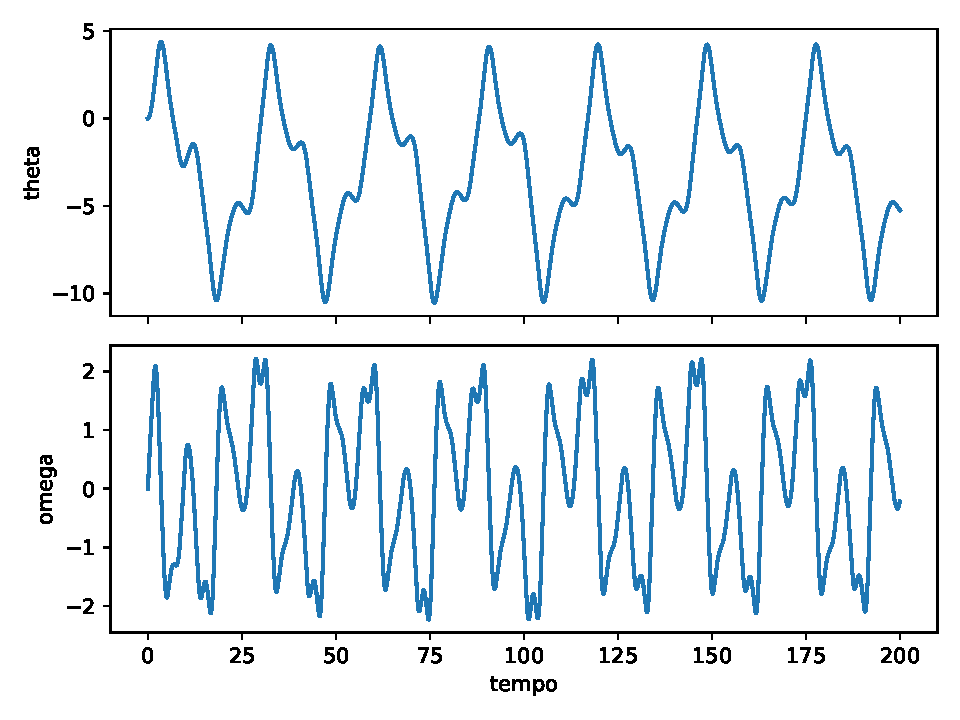
\includegraphics[width=0.7\linewidth]{figs/pendulo}
\end{figure}

\subsection{Método de Euler}
Equações diferenciais ordinárias podem ser resolvidas analiticamente (não abordado neste curso) ou numericamente. Dentre os vários métodos existentes para a solução numérica, a adotada aqui é o método de Euler. Considere a equação $\frac{dx}{dt}=f(x,t)$, com $f(x,t)$ uma função qualquer de $x$ em relação à $t$. Dado um valor inicial $x0$ (usualmente com $t=0$), é possível simular a equação usando pontos discretos com intervalos $\Delta t$ fixos. Cada valor $x_n$ é dado por $x_n=x(t_n=n\Delta t)$. A partir disso, é possível usar o método de Euler avançado para calcular um valor seguinte a partir do valor anterior, ou seja:
$$
x_{n+1}=x_n+f(x_n,t_n)\Delta t
$$

\begin{figure}[htb!]
	\centering
	\caption{Método de Euler}
	\label{fig:euler}
	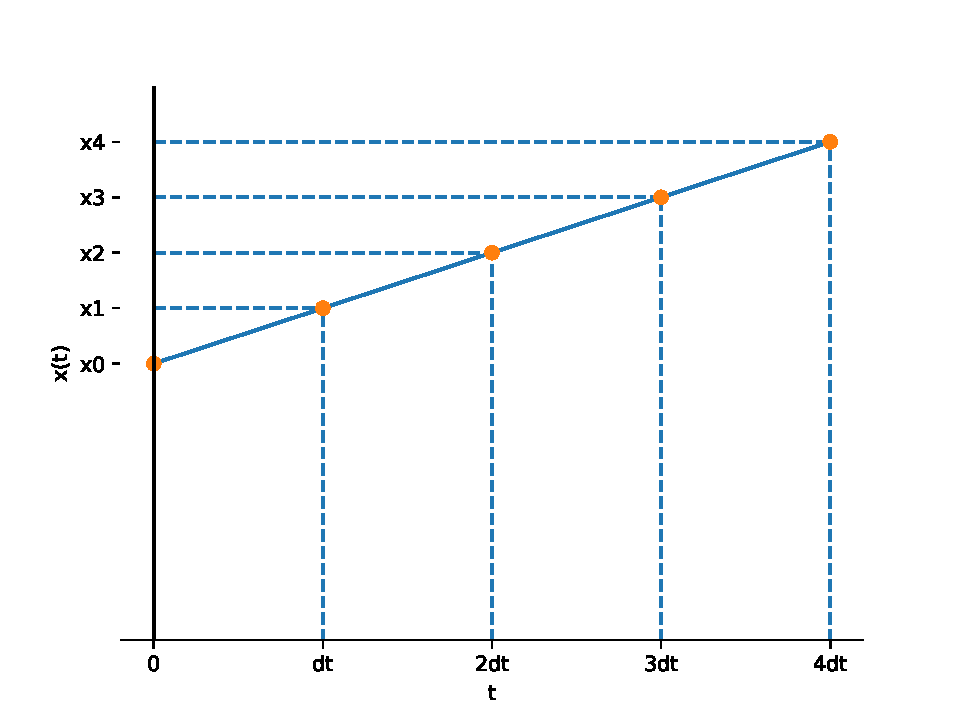
\includegraphics[width=0.7\linewidth]{figs/euler}
\end{figure}

Outros métodos não abordados no curso incluem o método de Euler reverso e o Runge-Kutta de segunda e quarta ordens, que são mais precisos na solução.

\section{Probabilidade}\label{sec:probabilidade}
\begin{itemize}
	\item Experimento aleatório: pode fornecer resultados diferentes a cada vez que se repete da mesma maneira
	\item Espaço amostral (S): conjunto de resultados possíveis para um experimento aleatório (pode ser contínuo ou discreto)
	\item Espaço amostral discreto: conjunto finito ou infinito contável de resultados
	\item Espaço amostral contínuo: intervalo (finito ou infinito) de números reais
	\item Evento (E): subconjunto do espaço amostral
\end{itemize}


\subsection{Probabilidade}
\begin{itemize}
	\item Probabilidade: quantifica a chance de ocorrer o resultado de um experimento aleatório (“A chance de chover hoje é de 30\%")
	\item Axiomas:
	\begin{enumerate}
		\item $P(S)=1$
		\item $0\leq P(E)\leq 1$
		\item $E_1\cap E_2=\emptyset\to P(E_1)+P(E_2)$
	\end{enumerate}
	\item Probabilidade da união: $P(A\cup B)=P(A)+P(B)-P(A\cap B)$
	\item Probabilidade condicional: $P(B|A)=P(A\cap B)/P(A),\quad P(A)>0$
	\item Teorema de Bayes:  $P(A|B)=\frac{P(B|A)P(A)}{P(B)},\quad P(B)>0$\\ % ex. do teste de droga
	\begin{description}
		\item[Exemplo:] Pelo fato de um novo procedimento médico ter se mostrado efetivo na detecção prévia de uma doença, propôs-se um rastreamento médico da população. A probabilidade de o teste identificar corretamente alguém com a doença, dando positivo, é $0,99$, e a probabilidade de o teste identificar corretamente alguém sem a doença, dando negativo, é $0,95$. A incidência da doença na população em geral é $0,0001$. Você fez o teste e o resultado foi positivo. Qual é a probabilidade de você ter a doença?
		\item[Solução:] Seja $D$ o evento em que você tem a doença e seja $S$ o evento é que o teste é positivo. A probabilidade requerida pode ser denotada como $P(D|S)$. A probabilidade de o teste identificar corretamente alguém sem a doença, dando negativo, é $0,95$. Consequentemente a probabilidade de um teste positivo sem a doença é
		$$P(S|D') = 0,05$$
		Do Teorema de Bayes,
		\begin{align*}
			P(D|S)&=P(S|D)P(D)/[P(S|D)P(D)+P(S|D')P(D')]\\
			&=0,99*0,0001/[0,99*0,0001+0,05*(1-0,0001)]\\
			&=1/506=0,002
		\end{align*}
		\item[Interpretação Prática:] A probabilidade de você ter a doença da de um resultado positivo do teste é somente 0,002. Surpreendentemente, embora o teste seja efetivo, no sentido de que $P(S|D)$ é alto e $P(S|D')$ é baixo, por causa da incidência da doença na população em geral ser baixa, as chances são bem pequenas de você realmente ter a doença, mesmo se o teste for positivo
	\end{description}
\end{itemize}


\subsection{Variáveis aleatórias}
\begin{itemize}
	\item Variável aleatória ($X$): função que atribui um número real ($x$) a cada resultado no espaço amostral de um evento aleatório
	\item Discretas: número de pessoas adultas em um ambiente; numero de carros em uma rodovia
	\item Contínuas: corrente elétrica; temperatura; tempo
	\item Função densidade de probabilidade discretas:
	\begin{enumerate}
		\item $f(x_i) \geq 0$ (para todo $x$)
		\item $\sum_{i=1}^n f(x_i)=1$
		\item $f(x_i)=P(X=x_i)$
	\end{enumerate}
	\item Função de distribuição cumulativa discretas: $F(x)=P(X\leq x)=\sum_{x_i\leq x}f(x_i)$
	\begin{enumerate}
		\item $0\leq F(x)\leq 1$
		\item Se $x\leq y$, então $F(x)\leq F(y)$
	\end{enumerate}
	\item Função densidade de probabilidade contínuas:
	\begin{enumerate}
		\item $f(x) \geq 0$ (para todo $x$)
		\item $\int_{-\infty}^\infty f(x)\mathrm{d}x=1$
		\item $P(a\leq X\leq b)=\int_a^b f(x)\mathrm{d}x=$ área sob $f(x)$ de $a$ a $b$ para qualquer $a$ e $b$
	\end{enumerate}
	\item Função de distribuição cumulativa contínuas: $F(x)=P(X\leq x)=\int_{-\infty}^{x}f(u)\mathrm{d}u$
\end{itemize}
\subsubsection{Média e variância}
\begin{itemize}
	\item Média (valor esperado) de uma variável aleatória discreta: $\mu=E(X)=\sum_{x}xf(x)$
	\item Variância de uma variável aleatória discreta: $\sigma^2=V(X)=E(X-\mu)^2$ (desvio-padrão: $\sigma=\sqrt{\sigma^2}$)
	\item Média (valor esperado) de uma variável aleatória contínua: $\mu=E(X)=\int_{\infty}^{\infty}xf(x)\mathrm{d}x$
	\item Variância de uma variável aleatória contínua: $\sigma^2=V(X)=\int_{-\infty}^{\infty}x^2f(x)\mathrm{d}x-\mu^2$ (desvio-padrão: $\sigma=\sqrt{\sigma^2}$)
\end{itemize}

\subsubsection{Distribuição de Poisson}
$$
f(x)=\frac{e^{-\lambda T}(\lambda T)^x}{x!}, x=0,1,2,\dots
$$
\begin{itemize}
	\item $T$: intervalo do evento
	\item $\lambda$: número médio de eventos por intervalo ($0\leq\lambda$)
	\begin{description}
		\item[Exemplo:] Falhas ocorrem ao acaso ao longo do comprimento de um fio delgado de cobre. Suponha que o número de falhas siga a distribuição de Poisson, com uma média de 2,3 falhas por milímetro. Determine a probabilidade de existirem exatamente duas falhas em 1 milímetro de fio.
		\item[Solução:] Seja $X$ o número de falhas em 1 milímetro de fio. Então, $E(X)=2,3$ falhas e
		$$P(X=2) = \frac{e^{-2,3}(2,3)^2}{2!}=0,265$$
		Para determinar a probabilidade de 10 falhas em 5 milímetros de fio, consideramos $X$ o número de falhas em 5 milímetros de fio. Então, $X$ tem uma distribuição de Poisson com
		$$\lambda T=5\text{ mm X }2,3\text{ falhas/mm}=11,5\text{ falhas}$$
		Consequentemente,
		$$P(X=10)=e^{-11,5}\frac{(11,5)^{10}}{10!}=0,113$$
		\item[Interpretação Prática:] Dadas as suposições para um processo de Poisson e um valor para $\lambda$, as probabilidades podem ser calculadas para intervalos arbitrários de comprimento.
	\end{description}
\end{itemize}

\subsubsection{Distribuição normal (Gaussiana)}
$$
f(x)=\frac{1}{\sqrt{2\pi\sigma}}e^{\frac{-(x-\mu)^2}{2\sigma^2}}\qquad-\infty<x<\infty
$$

$$
E(X)=\mu\qquad V(X)=\sigma^2
$$

\begin{figure}[htb!]
	\centering
	\caption{Funções densidade de probabilidade normal para diferentes valores de $\mu$ e $\sigma^2$}
	\label{fig:normal}
	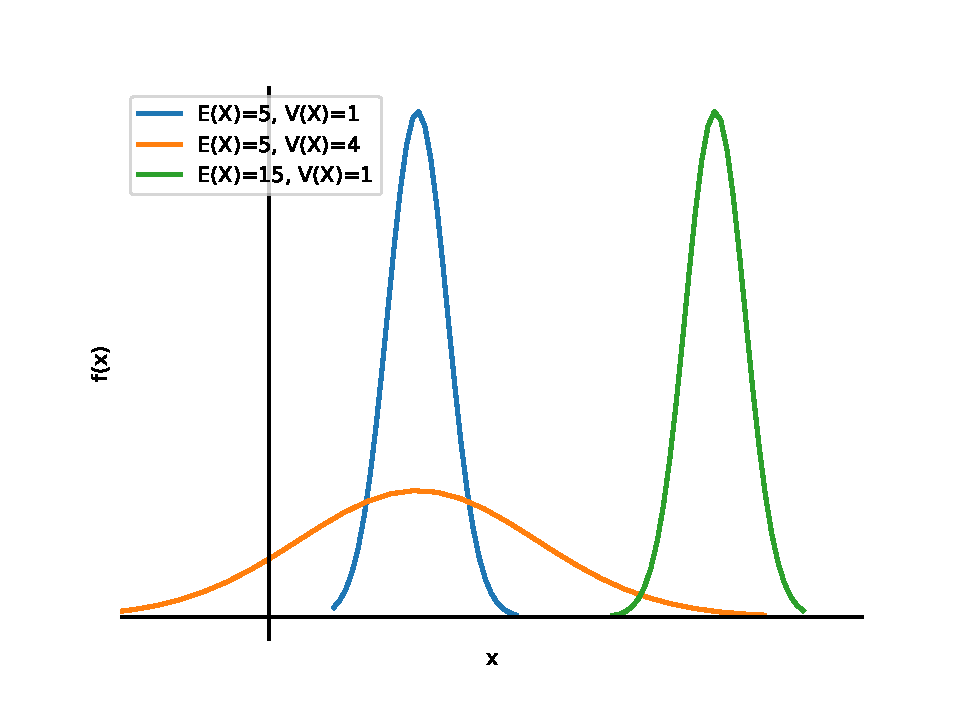
\includegraphics[width=0.7\linewidth]{figs/normal}
\end{figure}


\begin{itemize}
	\item Normal padrão: $\Phi(z)=P(Z\leq z)$, quando $\mu=0$ e $\sigma=1$
\end{itemize}


\section{Noções de algoritmos e programação}\label{sec:algoritmo}
\begin{itemize}
	\item \textbf{Algoritmo}: sequência de instruções para executar uma determinada tarefa. Ex.: algoritmo para lavar as mãos
	\begin{enumerate}
		\centering
		\item Início
		\item Abrir a torneira
		\item Molhar as mãos
		\item Ensaboar as mãos
		\item Molhar as mãos
		\item Secar as mãos
		\item Fim
	\end{enumerate}
	
	\item \textbf{Programa}: conjunto de instruções escritas em um arquivo com regras específicas
	\begin{verbatim}
		print("Olá, mundo!")
	\end{verbatim}
	\item \textbf{Linguagem de programação}: converte o programa escrito em ações no computador (ex.: \textit{Python}, \textit{C++}, \textit{Java})
\end{itemize}

\begin{figure}[htb!]
	\centering
	\caption{Do código para e/s}
	\label{fig:codigoio}
	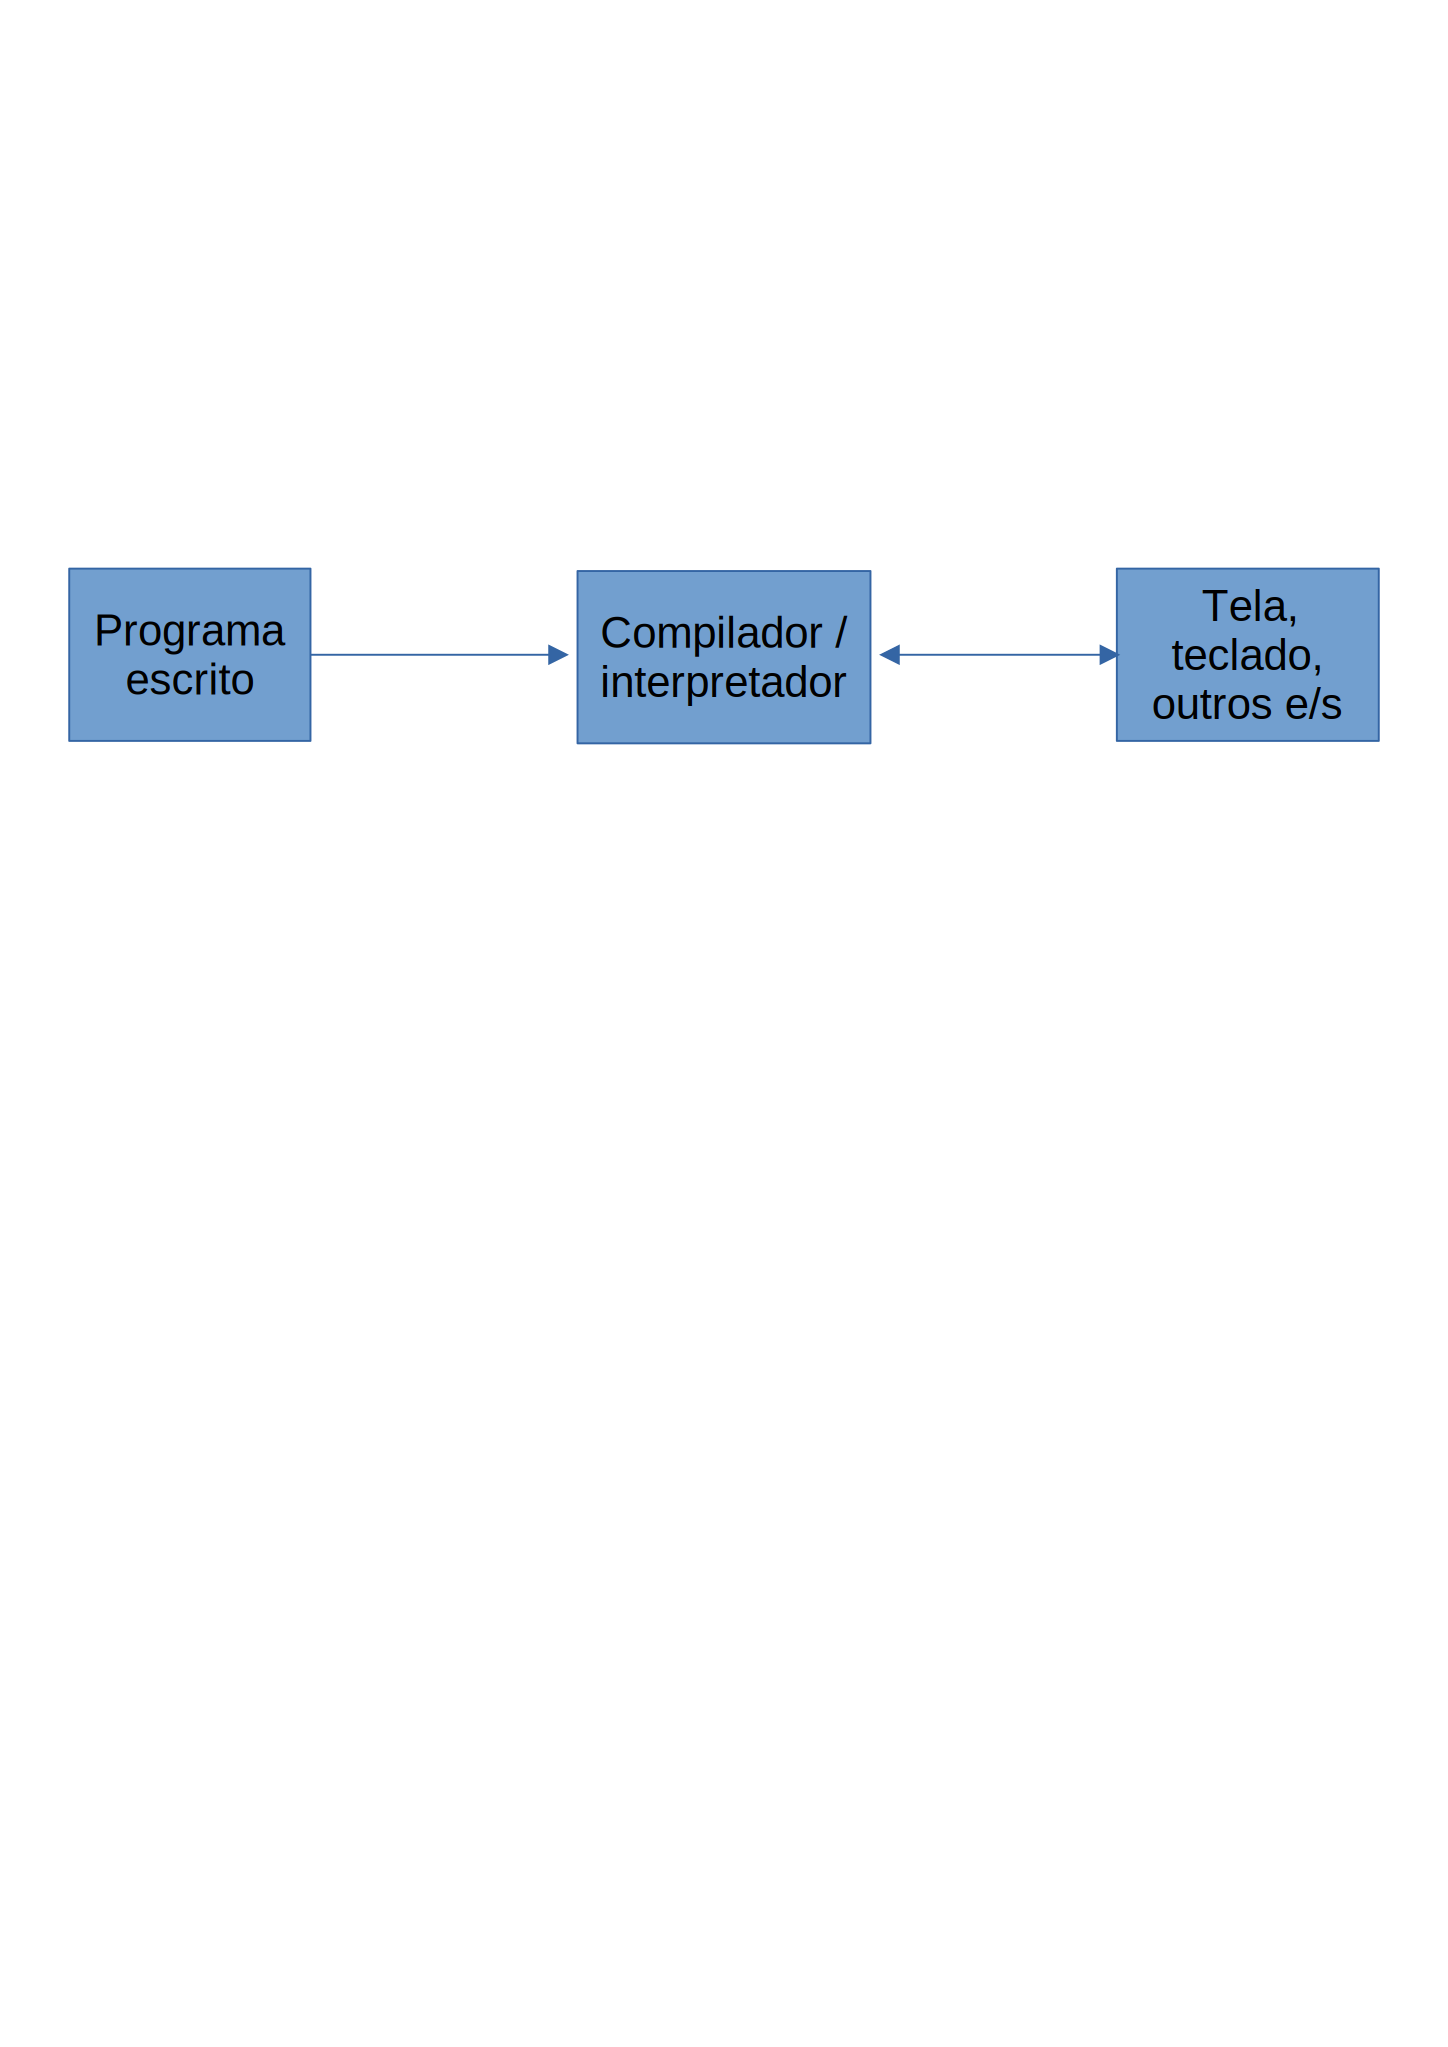
\includegraphics[width=0.7\linewidth]{figs/codigo_io}
\end{figure}

\SetKwComment{Comment}{/* }{ */}
\begin{algorithm}
	\caption{Exemplo}\label{alg:ohm}
	\KwData{$n \geq 0$}
	\KwResult{$y = x^n$}
	$y \gets 1$\;
	$X \gets x$\;
	$N \gets n$\;
	\While{$N \neq 0$}{
		\eIf{$N$ é par}{
			$X \gets X \times X$\;
			$N \gets \frac{N}{2}$ \Comment*[r]{Este é um comentário}
		}{\If{$N$ é impar}{
				$y \gets y \times X$\;
				$N \gets N - 1$\;
			}
		}
	}
\end{algorithm}

\chapter{Modelos de neurônio}\label{cap:modelos}
\section{Introdução}\label{sec:modelos_intro}
Os modelos são formas de representar, matemática e/ou computacionalmente, o comportamento do neurônio. Os modelos podem variar desde os mais simples, que não representam fielmente o comportamento fisiológico do neurônio mas são úteis para simular grandes quantidades de neurônios, até os mais complexos, que trazem diversas representações de condutância e morfológicas. Alguns modelos de neurônio são apresentados na Tabela~\ref{tab:modelos_neuronios}, incluindo o número de variáveis presentes no modelo, o que reflete o número de equações diferenciais presentes e, consequentemente, a complexidade do mesmo, bem como é informado se o modelo é considerado biologicamente plausível. Os 4~(quatro) primeiros modelos são detalhados neste texto, por hora diferenciados entre os que simulam o disparo do potencial de ação, chamados aqui de modelos de disparo de neurônio, e os que simulam a taxa de disparo. Há, ainda, distinção, por exemplo, entre modelos de compartimento único, que modelam o potencial de membrana apenas pela variável $V$, e os multi-compartimento, que consideram variações espaciais no potencial de membrana, porém estes últimos não são abordados neste texto.

\begin{table}
	\IBGEtab{
	\centering
	\caption[Modelos de neurônio]{Modelos de neurônio}
	\label{tab:modelos_neuronios}
	}{
	\begin{tabular}{|c|c|c|c|}
		\hline
		Modelo & N. variáveis & Complexidade & Biol. plausível \\
		\hline
		Leaky integrate-and-fire & 1 & Muito baixa & Não \\
		\hline
		Izhikevich & 2 & Muito baixa & Não \\
		\hline
		Hodgkin-Huxley & 4 & Muito alta & Sim \\
		\hline
		Wilson-Cowan & 2 & Média & Não \\
		\hline
		Spike response model & 1 & Baixa & Não \\
		\hline
		FitzHugh-Nagumo & 2 & Média & Não \\
		\hline
		Moris-Lecar & 3 & Alta & Sim \\
		\hline
	\end{tabular}
}{
\fonte{O autor (2023)}
}
\end{table}

\section{Modelos de disparo de neurônios}\label{sec:modelosdisparo}
\subsection{Modelo integra-e-dispara com vazamento}\label{sec:modelolif}

Para modelos de neurônio de compartimento único, o circuito elétrico equivalente da membrana pode ser representado como na Figura~\ref{fig:circuitomembrana}.
\begin{figure}[htb!]
	\centering
	\caption{Circuito equivalente da membrana}
	\label{fig:circuitomembrana}
	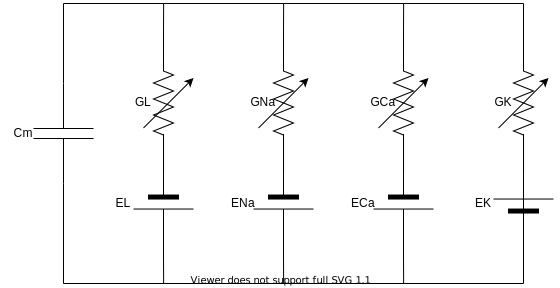
\includegraphics[width=0.7\linewidth]{figs/circuito_membrana}\\
\end{figure}
O capacitor na esquerda está associado à capacitância da membrana ($C_m$), e cada resistor em série com uma bateria representa um canal iônico. A série com o $L$ subscrito refere-se ao elemento de vazamento, citado anteriormente, e as séries são referentes aos canais iônicos dependentes de tensão, com o íon subscrito. O circuito completo tem associada a seguinte equação:
\begin{equation}\label{eq:potencial_membrana_total}
	c_m\frac{\mathrm{d}V_m}{\mathrm{d}t}=G_{Na}(E_{Na}-V_m)+G_{Ca}(E_{Ca}-Vm)+G_K(E_K-V_m)+G_L(E_L-V_m)
\end{equation}
sendo $G_A$ a condutância do íon $A$, $E_A$ o potencial do íon $A$. Ignorando por hora os canais iônicos dependentes de tensão, a equação fica como a \ref{eq:potencial_membrana}. Adicionando-se a corrente aplicada, incluímos também uma condição que força o disparo do potencial de ação quando o potencial de membrana atinge um determinado limitar ($V_{th}$), forçando o potencial de membrana para um valor de \textit{reset} ($V_{reset}$) \cite{miller_introductory_2018}. Com isso, o circuito fica equivalente à Figura~\ref{fig:circuitolif} e a equação total é como abaixo.
\begin{equation}\label{eq:lif}
	c_m\frac{dV_m}{dt} = G_L(E_L-V_m)+I_{ap}; \text{ se } V_m > V_{th} \text{ então } V_m\mapsto V_{reset}
\end{equation}
\begin{figure}[htb!]
	\centering
	\caption{Circuito equivalente do modelo LIF}
	\label{fig:circuitolif}
	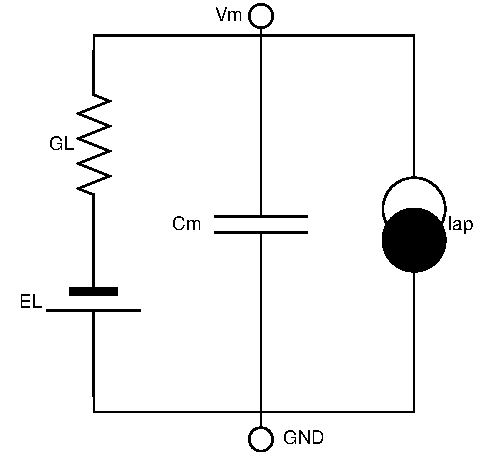
\includegraphics[width=0.5\linewidth]{figs/circuito_lif}
\end{figure}
Essa é a equação do modelo \textit{Leaky integrate-and-fire} (integra e dispara com vazamento, em tradução livre) \cite{lapicque_recherches_1907}. A corrente aplicada no modelo é acumulada (integrada), elevando o potencial de membrana até o valor de limiar, representando o momento onde o neurônio dispara. Devido a simplicidade do modelo, a equação, por si só, não é capaz de representar a hiperpolarização que ocorre fisicamente na célula neuronal após o disparo do potencial de ação, e, por isso, é acrescentada a condição de \textit{reset}. Enquanto a corrente continuar sendo aplicada, o potencial de membrana permanece sendo atualizado pela dinâmica da equação diferencial, como é exibido na Figura~\ref{fig:lif}. Três pulsos de corrente, com valores $0,18\ nA$, $0,21\ nA$ e $0,24\ nA$, são aplicados no modelo. Para o primeiro valor, o neurônio despolariza (fica menos negativo), porém não atinge o valor de limiar (como visto na primeira curva da segunda linha de gráficos). Com a injeção dos demais valores de corrente, a célula neuronal atinge o valor de limiar ($50\ mV$ nestes exemplos), ocorrendo o disparo do potencial de ação (registrado como uma linha vertical na última linha de gráficos), e com a posterior alteração do potencial de membrana para o valor de \textit{reset} ($80\ mV$ nestes exemplos).

\begin{figure}[htb!]
	\centering
	\caption[Exemplo da simulação com o modelo LIF]{Exemplo da simulação com o modelo LIF. Cada coluna representa um valor diferente de corrente aplicada ao modelo, que são mostradas na primeira linha de gráficos. Na segunda linha são exibidos os potenciais de membrana para cada corrente injetada. Em baixo, os instantes em que ocorreu o disparo de potenciais de ação.}
	\label{fig:lif}
	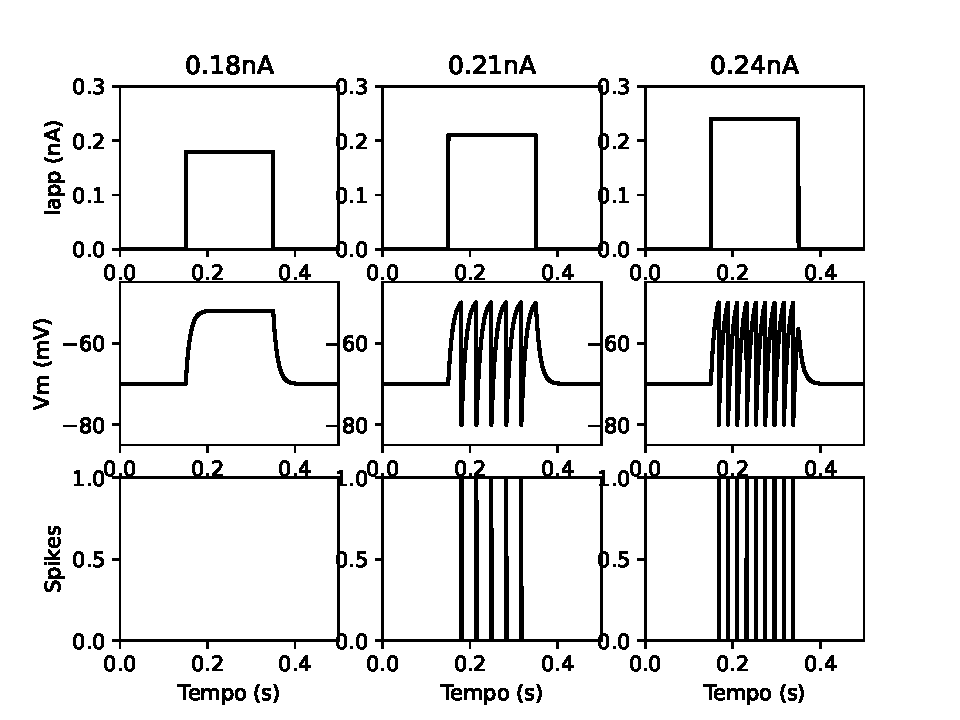
\includegraphics[width=0.7\linewidth]{figs/lif}
\end{figure}

%% incluir a solução analítica para enfatizar a presença da constante de tempo

\subsection{Extensões do modelo LIF}
Apesar de útil e ser utilizado em inúmeras simulações neuronais, o modelo LIF é carente de diversos comportamentos presentes fisiologicamente no neurônio. Algumas delas são apresentadas aqui como extensões ao modelo, a fim de acrescentar algumas características que podem ser úteis nas simulações. As extensões apresentadas simulam a refratariedade e a adaptação da taxa de disparo, além de versões do modelo LIF com componentes exponenciais e adaptativas, como mostradas na sequência.
\subsubsection{Período refratário}
Imediatamente após a ocorrência do potencial de ação, o neurônio não é capaz de produzir um novo potencial de ação durante um curto período de tempo, e esse tempo é chamado de período refratário. Existem diferentes métodos para simular esse comportamento nos modelos neuronais, e aqui mostramos três, acrescentadas ao modelo LIF, com os seus comportamentos exibidos na Figura~\ref{fig:lifrefratario}.
\begin{figure}[tb]
	\centering
	\caption{Simulação do modelo LIF com período refratário}
	\label{fig:lifrefratario}
	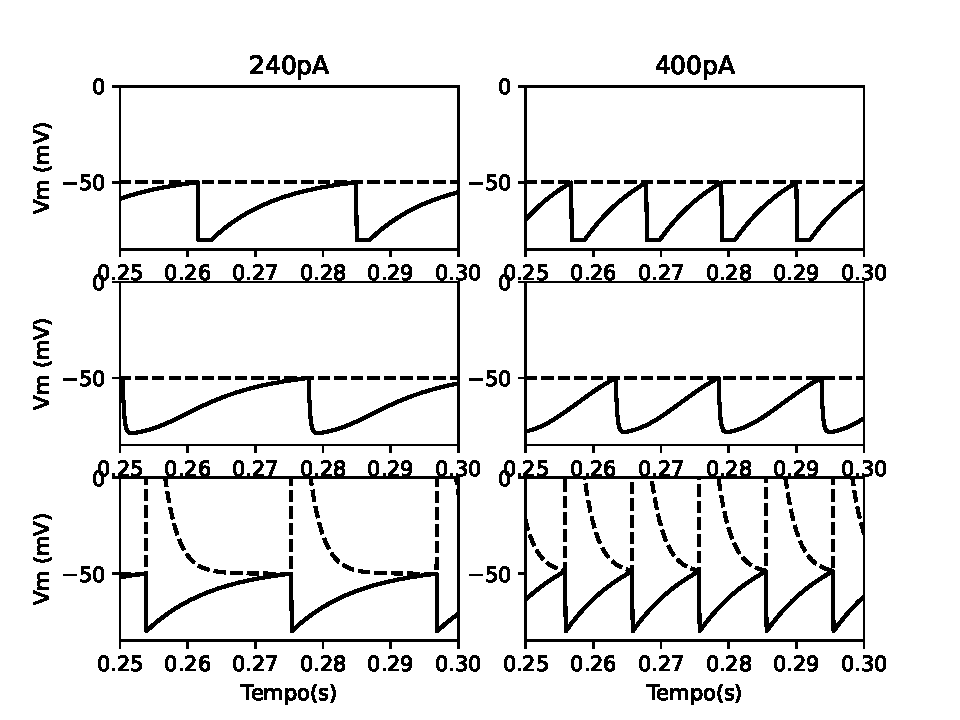
\includegraphics[width=0.7\linewidth]{figs/lif_refratario}
\end{figure}
Em todos os métodos são simuladas a injeção de corrente de $240\ pA$ (primeira coluna de gráficos) e $400\ pA$ (segunda coluna), e a linha tracejada representa o limiar para disparo do potencial de ação. O primeiro método é chamado de \textbf{grampeamento de tensão},que consiste em fixar o potencial de membrana no valor de \textit{reset} durante um tempo específico logo após o potencial de ação. É, provavelmente, a maneira mais simples de simular a refratariedade, pois neste método o período refratário é constante. O segundo método é o da \textbf{condutância refratária}, consistindo no acréscimo de uma condutância elevada, geralmente uma corrente hiperpolarizante de potássio, que cresce imediatamente após a ocorrência de cada potencial de ação, e decai em seguida de acordo com a seguinte equação diferencial:
\begin{equation}\label{eq:condutancia_refrataria}
	\frac{dG_{ref}(t)}{dt} = -\frac{G_{ref}(t)}{\tau_{ref}};\text{ depois do potencial de ação } G_{ref} \mapsto G_{ref} + \Delta G
\end{equation}
sendo $\tau_{ref}$ a constante de tempo do período refratário e $\Delta G$ o incremento de condutância. Como visto na segunda linha de gráficos, o potencial de membrana cresce em um ritmo mais lento que o normal, devido à corrente de potássio que hiperpolariza a célula. Essa corrente é representada acrescentando-se à parte direita da equação do modelo LIF o termo $G_{ref}(t)[E_k-V_m(t)]$, com $E_k$ sendo o potencial de reversão para os íons de potássio (como na Tabela~\ref{tab:concentracao_nernst}). O último método é chamado de \textbf{incremento do limiar}, onde é elevado, após cada potencial de ação, o limiar necessário para ocorrer um novo disparo. Esse limiar decai conforme a equação:
\begin{equation}\label{eq:incremento_limiar}
	\frac{dV_{th}(t)}{dt} = \frac{V^0_{th}-V_{th}(t)}{\tau_{ref}};\text{ depois do potencial de ação } V_{th} \mapsto V_{th} + \Delta V
\end{equation}
sendo $V^0_{th}$ o potencial de limiar de referência (o valor do limiar em repouso). Como visto na última linha de gráficos, o limiar (linha tracejada) cresce absurdamente após cada disparo de potencial de ação, decaindo logo em seguida, ao contrário do potencial de membrana, que decai e cresce em seguida. 

\subsubsection{Adaptação da taxa de disparos}
Uma característica presente nos neurônios é a sua capacidade de adaptar a frequência em que os disparos de potencial de ação ocorrem, com uma diminuição da taxa logo após o primeiro disparo. Uma fácil percepção da consequência da adaptação da taxa de disparo é a diferença de percepção de cheiros intensos ao longo do tempo, como quando uma pessoa entra com um perfume forte em um elevador. A implementação da adaptação da taxa de disparos é feita de maneira semelhante ao método da condutância refratária apresentada anteriormente, porém com duas diferenças:
\begin{itemize}
	\item O incremento da condutância é menor em comparação ao do período refratário. Esse incremento menor não impede o disparo de novos potenciais (o que acontece no período refratário), porém diminui a taxa deles
	\item A escala de tempo (a constante) da condutância adaptativa é bem maior, o que permite o acúmulo das condutâncias ao longo da sequência de disparos
\end{itemize}
A dinâmica da adaptação da taxa de disparos é exibida na Figura~\ref{fig:lifatd}. Como no exemplo do período refratário, correntes de $240\ pA$ e $400\ pA$ são injetadas, sendo exibidas as curvas de potencial de membrana (em cima), e da condutância adaptativa (embaixo), onde se pode observar incremento e acúmulo de condutância.

\begin{figure}[tb]
	\centering
	\caption{Adaptação da taxa de disparo no neurônio LIF}
	\label{fig:lifatd}
	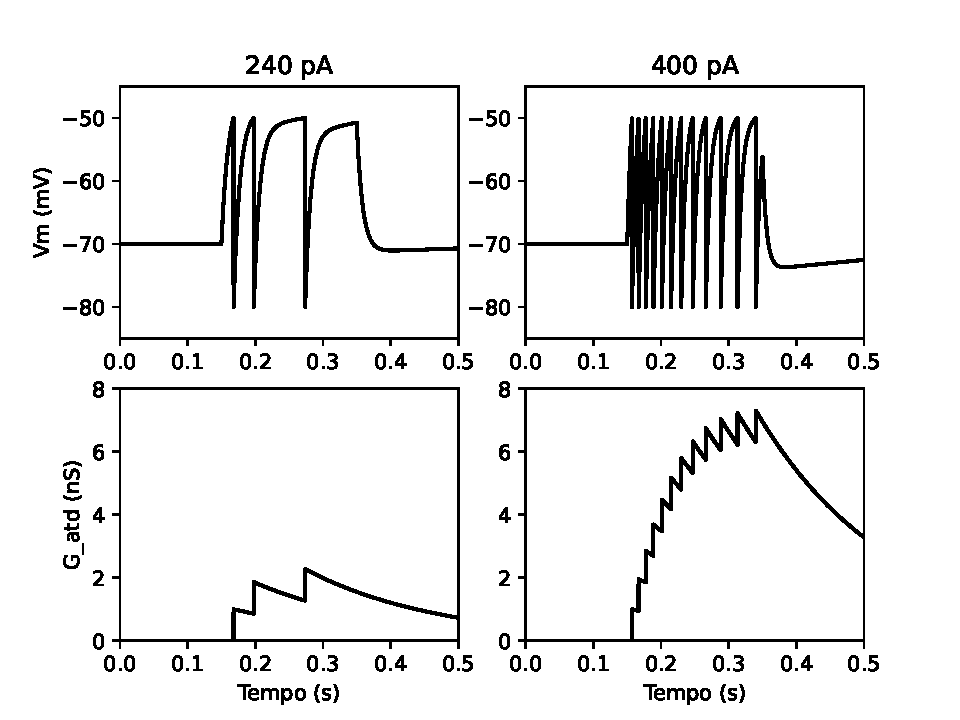
\includegraphics[width=0.7\linewidth]{figs/lif_atd}
\end{figure}

\subsubsection{Modelo LIF exponencial}
O modelo LIF exponencial (ELIF) incorpora um termo adicional para a geração do potencial de ação, que é uma falta existente no modelo tradicional. Esse termo acrescenta uma corrente despolarizante, elevando quase que instantaneamente o valor do potencial de membrana quando este se aproxima do limiar. Esse crescimento tende ao infinito, porém nas simulações é definido um limite ($V_{max}$), devido o computador ter problemas para lidar com valores infinitos, alterando a condição do modelo para a equação abaixo:
\begin{equation}\label{eq:elif_cond}
	\text{se } V_m > V_{max} \text{ então } V_m\mapsto V_{reset}
\end{equation}
Além disso, não há exatamente um valor fixo para o disparo do potencial, e sim um intervalo ($\Delta_{th}$), e a equação completa deste modelo fica:
\begin{equation}\label{eq:elif}
	c_m\frac{dV_m}{dt} = G_L(E_L-V_m) + G_L\Delta_{th}\exp\Big(\frac{V_m-V_{th}}{\Delta_{th}}\Big) + I_{ap}
\end{equation}
Os gráficos comparando o potencial de membrana do modelo LIF (em cima) e ELIF (embaixo) são mostrados na Figura~\ref{fig:elif}. Uma característica interessante é a inflexão presente no modelo ELIF quando o potencial de membrana se aproxima do instante em que ocorre o disparo do potencial de ação, algo inexistente no modelo LIF.

\begin{figure}[tb]
	\centering
	\caption{Comparação dos modelos LIF e ELIF}
	\label{fig:elif}
	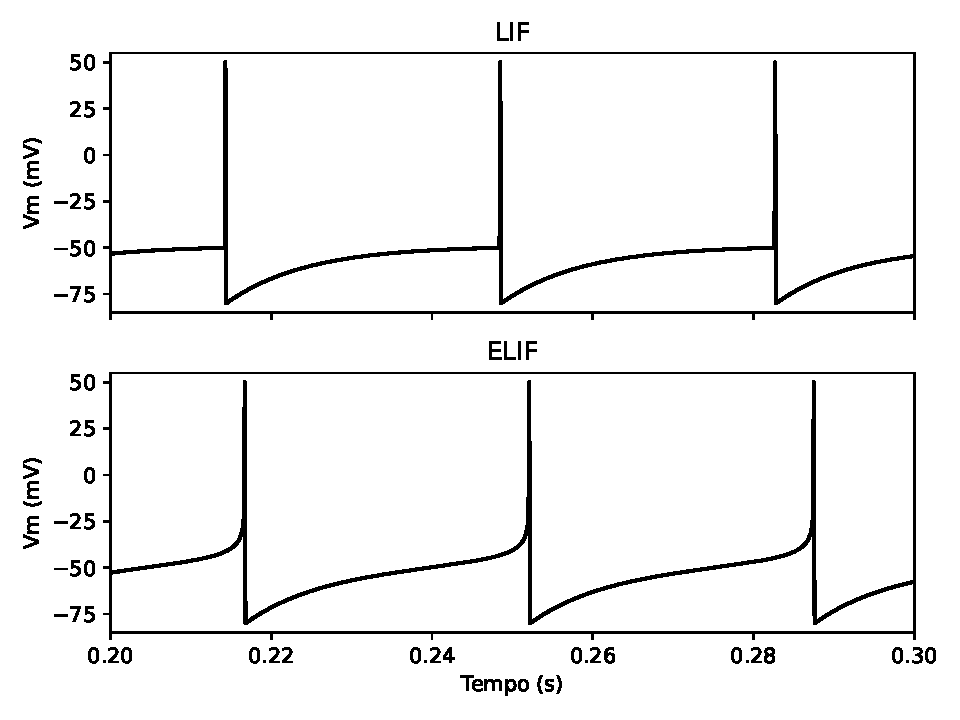
\includegraphics[width=0.7\linewidth]{figs/elif}
\end{figure}

\subsubsection{Modelo LIF exponencial adaptativo}
O modelo LIF exponencial adaptativo (AELIF) adiciona uma corrente adaptativa hiperpolarizante ao modelo anterior, similar à utilizada no método da condutância refratária, porém com o decaimento dependendo do potencial de membrana. É um modelo com duas equações, sendo uma para a variável de adaptação ($w$) e a outra para o potencial de membrana, que é semelhante à do modelo anterior, e ambas tem um \textit{reset} quando ocorre o disparo do potencial de ação.
% Esse modelo é capaz de descrever padrões de disparo comuns, como \textit{bursting, fast spiking, regular spiking}, dentre outros.
As equação para este modelo são:
\begin{equation}
	c_m\frac{dV_m}{dt} = G_L(E_L-V_m) + G_L\Delta_{th}\exp\Big(\frac{V_m-V_{th}}{\Delta_{th}}\Big) - w + I_{ap}
\end{equation}
\begin{equation}
	\tau_w\frac{dw}{dt}=a(V_m-E_L)-w
\end{equation}
com as condições:
\begin{equation}
	\text{se } V_m > V_{max} \text{ então } V_m\mapsto V_{reset} \text{ e } w\mapsto w + b
\end{equation}
sendo $a$ o parâmetro de agrupamento, indicando o nível de relação entre o potencial de membrana e a variável de adaptação, e $b$ o parâmetro de adaptação, que é o valor do incremento de corrente após o disparo do potencial de ação. A dinâmica do modelo ELIF é mostrada na Figura~\ref{fig:elif}, com o potencial de membrana exibido em cima e a variável de adaptação embaixo. É possível notar a semelhança da curva de adaptação com a da condutância adaptativa da adaptação da taxa de disparo, também semelhante ao método da condutância refratária.

\begin{figure}[tb]
	\centering
	\caption[Resposta do modelo AELIF]{Resposta do modelo AELIF para um pulso de corrente de 1 $nA$}
	\label{fig:adexrs}
	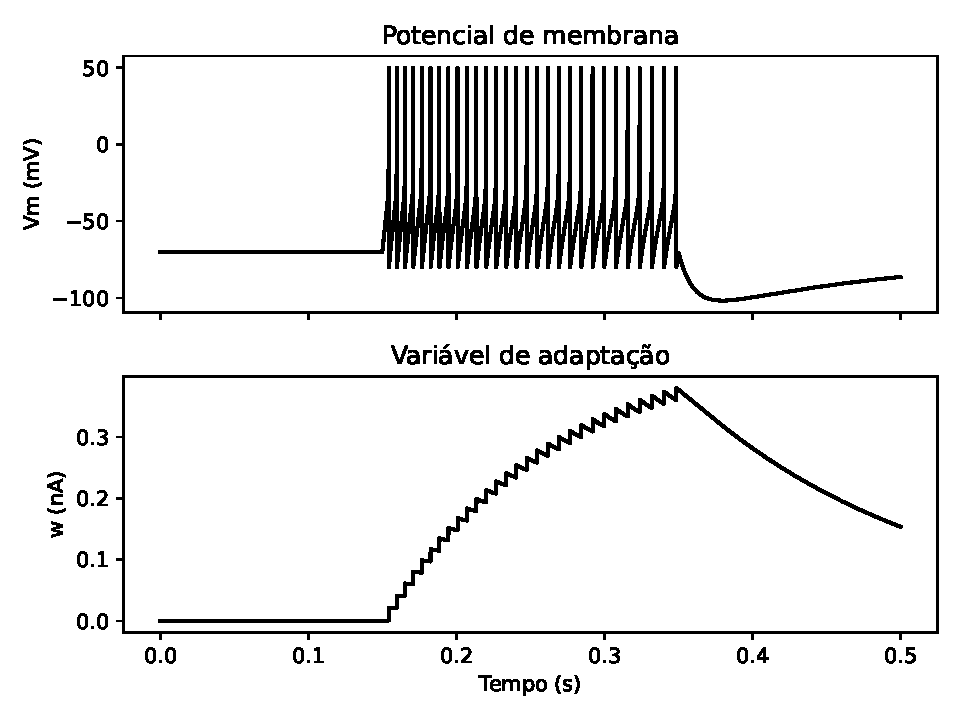
\includegraphics[width=0.7\linewidth]{figs/aelif}\\
\end{figure}

\subsection{Modelo de Izhikevich}\label{sec:izhikevich}
Em 2003, Eugene Izhikevich publicou um modelo capaz de simular vários comportamentos de neurônios corticais, combinando a plausabilidade biológica do modelo de Hodgkin-Huxley (que será visto na sequência) com a eficiência computacional do modelo LIF \cite{izhikevich_simple_2003}. Ele é composto por duas equações diferenciais, que são as seguintes:
\begin{equation}\label{eq:izhikevich_v}
	v'=0.04v^2+5v+140-u+I
\end{equation}
\begin{equation}\label{eq:izhikevich_u}
	u'=a(bv-u)
\end{equation}
com as condições de \textit{reset}
\begin{equation}\label{eq:izhikevich_condicao}
	\text{se }v\geq30\ mV,\text{ então }\begin{cases}
		v\leftarrow c\\
		u\leftarrow u+d
	\end{cases}
\end{equation}
com $v$ sendo o potencial de membrana, $u$ a variável de recuperação da membrana, e $I$ sendo a corrente injetada (a notação adotada aqui é a mesma usada por Izhikevich). Na Figura~\ref{fig:izhikevich} é exibido o potencial de membrana para um comportamento do tipo \textit{regular spiking} quando é injetada uma corrente de $10\ mA$.
\begin{figure}[tb]
	\centering
	\caption[Potencial de membrana no modelo de Izhikevich]{Potencial de membrana no modelo de Izhikevich}
	\label{fig:izhikevich}
	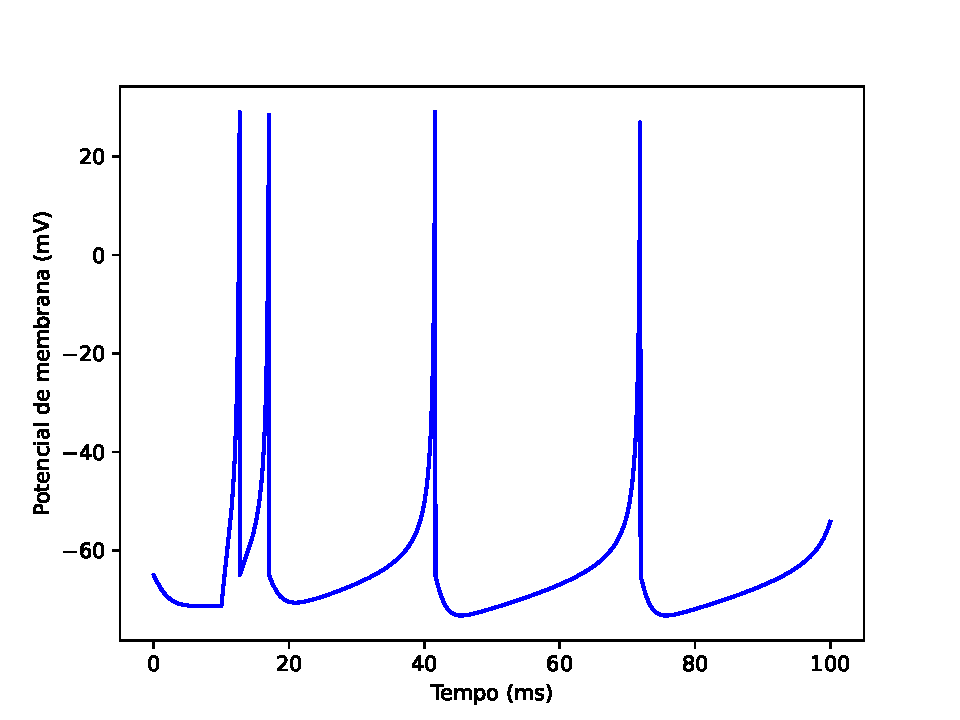
\includegraphics[width=0.7\linewidth]{figs/izhikevich}
\end{figure}
Os parâmetros \textit{a}, \textit{b}, \textit{c} e \textit{d} são definidos como segue:
\begin{itemize}
	\item O parâmetro \textit{a} representa a escala de tempo da variável de recuperação, onde valores pequenos resultam em uma recuperação mais lenta
	\item O parâmetro \textit{b} representa a sensibilidade da variável de recuperação às subflutuações do potencial de membrana, onde valores maiores agrupam mais $v$ e $u$
	\item O parâmetro \textit{c} representa o valor de \textit{reset} do potencial de membrana após o disparo do potencial de ação
	\item O parâmetro \textit{d} representa o valor de \textit{reset} da variável de recuperação após o disparo do potencial de ação
\end{itemize}
A combinação de determinados valores para os parâmetros acima produz saídas compatíveis com alguns dos comportamentos citados anteriormente, conforme listado na Tabela~\ref{tab:padroes_izhikevich}.
\begin{table}
	\IBGEtab{
	\centering
	\caption[Padrões de neurônio do modelo de Izhikevich]{Padrões de neurônio do modelo de Izhikevich}
	\label{tab:padroes_izhikevich}
	}{
	\begin{tabular}{|c|c|c|c|c|}
		\hline
		Padrão & a & b & c & d \\
		\hline
		\textit{regular spiking} & 0,02 & 0,2 & -65 & 8 \\
		\hline
		\textit{intrinsically bursting} & 0,02 & 0,2 & -55 & 4 \\
		\hline
		\textit{chattering} & 0,02 & 0,2 & -50 & 2 \\
		\hline
		\textit{fast spiking} & 0,1 & 0,2 & -65 & 2 \\
		\hline
		\textit{thalamo-cortical} & 0,02 & 0,25 & -65 & 0,05 \\
		\hline
		\textit{resonator} & 0,1 & 0,25 & -65 & 2 \\
		\hline
		\textit{low-threshold spiking} & 0,02 & 0,25 & -65 & 2 \\
		\hline
	\end{tabular}
}{
	\fonte{O autor, baseado em \cite{izhikevich_simple_2003}}
}
\end{table}

\subsection{Modelo de Hodgkin-Huxley}\label{sec:modelohh}
O último dos modelos de disparo de neurônio visto neste texto é o de Hodgkin-Huxley.
%TODO: citação
Como visto na Seção~\ref{sec:fisiologia}, existem canais iônicos que são dependente de tensão. A probabilidade de abertura desses canais é modificada em função do potencial de membrana. O mecanismo de funcionamento deles é como mostrado na Figura~\ref{fig:canais}. À esquerda, é possível ver os elementos que compõem esse tipo de canal: um sensor, que identifica o potencial de membrana; um filtro de seletividade, que seleciona apenas íons compatíveis com aquele canal; e os portões, que permitem ou não a passagem dos íons. Há dois tipos de portões, que estão relacionados aos processos de \textbf{ativação} e \textbf{inativação}. O primeiro refere-se à abertura de um canal iônico, geralmente devido à despolarização, que aumenta a probabilidade de um canal estar aberto. O seu oposto é a \textbf{desativação}, que fecha o canal, geralmente por hiperpolarização. A inativação é o processo que impede a abertura dos canais, tendo como oposto, necessário para que o canal se abra, chamado de \textbf{desinativação}.
\cite{miller_introductory_2018}
\begin{figure}[htb!]
	\centering
	\caption{Mecanismo de funcionamento dos canais iônicos dependentes de tensão}
	\label{fig:canais}
	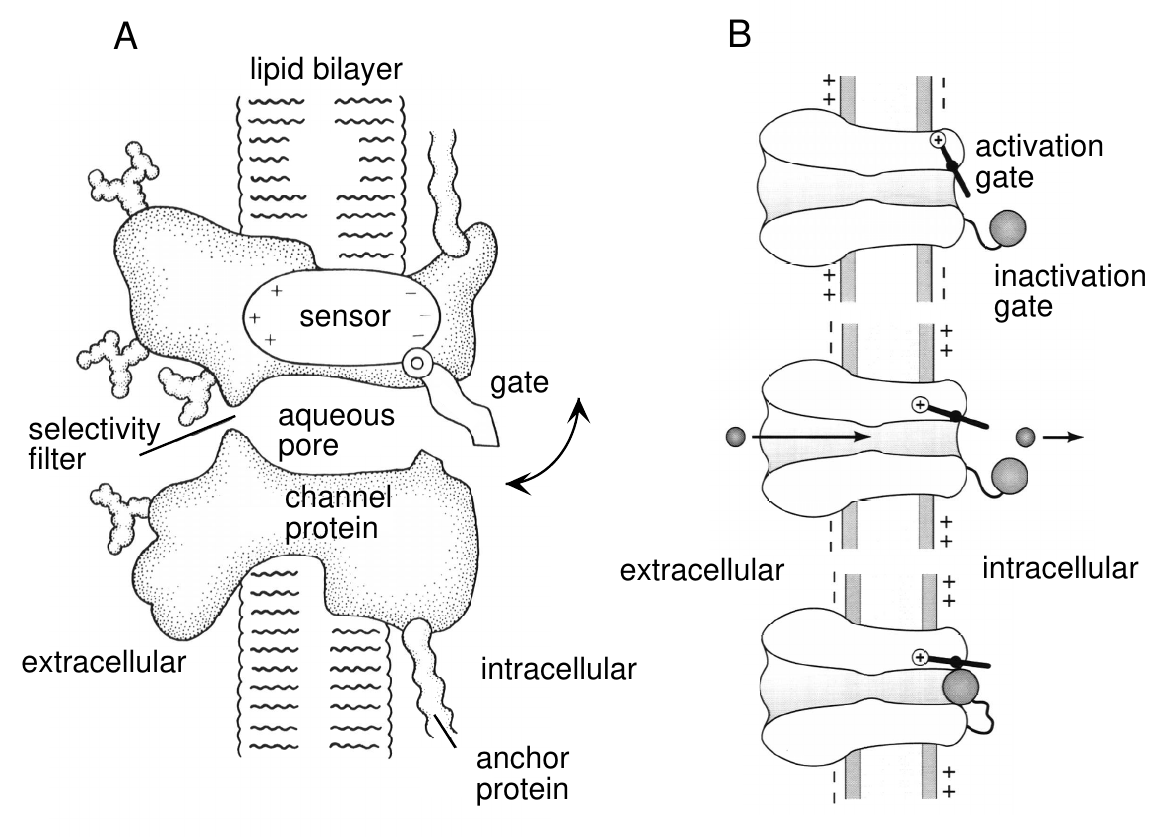
\includegraphics[width=0.6\linewidth]{figs/canais}\\
	\small{Fonte: \cite{dayan_theoretical_2001}}
\end{figure}
Associado aos canais iônicos dependentes de tensão, existe a chamada \textbf{variável de portão}, que representa a fração desses canais que se encontra em um determinado estado (ativado/desativado, inativado/desinativado). Como se trata da probabilidade do canal estar em um desses estados, seus valores são entre $0$ e $1$. No modelo, são consideradas as variáveis \textbf{m} para ativação de sódio, \textbf{h} para inativação de sódio, e \textbf{n} para ativação de potássio, com as equações a seguir:
\begin{equation}\label{eq:dmdt}
	\frac{dm}{dt}=\alpha_m(1-m)-\beta_mm
\end{equation}
\begin{equation}\label{eq:dhdt}
	\frac{dh}{dt}=\alpha_h(1-h)-\beta_hh
\end{equation}
\begin{equation}\label{eq:dndt}
	\frac{dn}{dt}=\alpha_n(1-n)-\beta_nn
\end{equation}
sendo $\alpha$ a constante de crescimento de cada variável, e $\beta$ a de decrescimento, ambas também dependentes de tensão, conforme as equações abaixo:
\begin{equation}\label{eq:alpha_m}
	\alpha_m=\frac{10^5(-V_m-0.045)}{\exp[100(-V_m-0.045)]-1}
\end{equation}
\begin{equation}\label{eq:beta_m}
	\beta_m=4*10^5\exp\Big[\frac{(-V_m-0.070)}{0.018}\Big]
\end{equation}
\begin{equation}\label{eq:alpha_h}
	\alpha_h=70\exp[50(-V_m-0.070)]
\end{equation}
\begin{equation}\label{eq:beta_h}
	\beta_h=\frac{10^3}{1+\exp[100(-V_m-0.040)]}
\end{equation}
\begin{equation}\label{eq:alpha_n}
	\alpha_n=\frac{10^4(-V_m-0.060)}{\exp[100(-V_m-0.060)]-1}
\end{equation}
\begin{equation}\label{eq:beta_n}
	\beta_n=125\exp\Big[\frac{(-V_m-0.070)}{0.08}\Big]
\end{equation}
\begin{figure}[tb]
	\centering
	\caption{Dinâmica das variáveis de portão}
	\label{fig:portoes}
	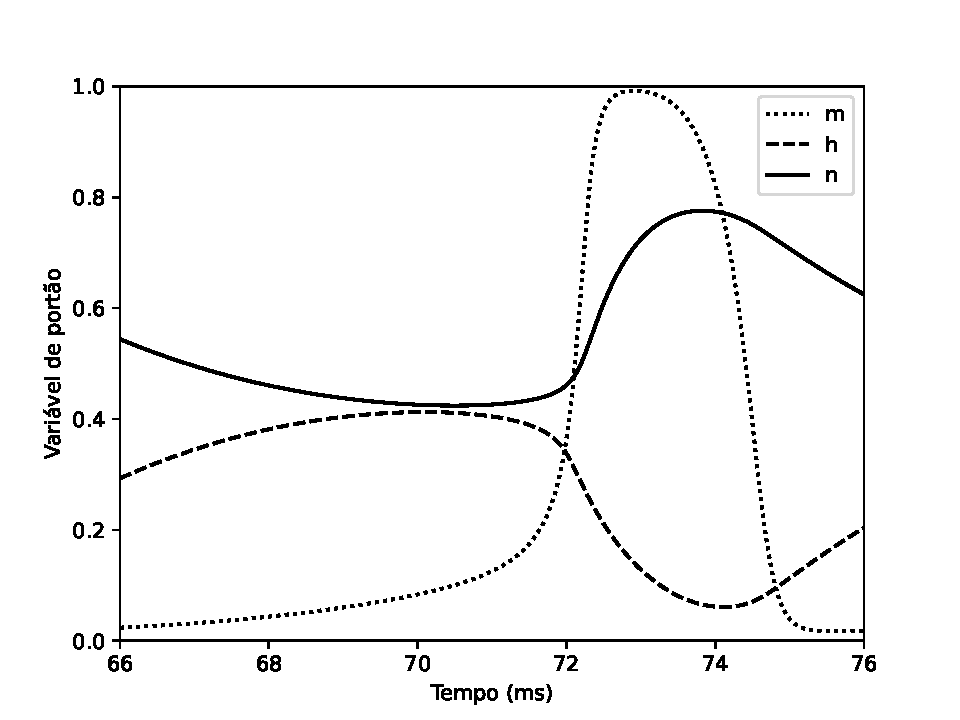
\includegraphics[width=0.7\linewidth]{figs/portoes}
\end{figure}
A dinâmica das variáveis de portão no modelo de Hodgkin-Huxley pode ser vista na Figura~\ref{fig:portoes}, para uma faixa de 66 até $76\ ms$. As variáveis de portão também podem se definidas pelas suas equações em \textbf{regime permanente}, que é o comportamento em repouso depois de um longo período de tempo \cite{ermentrout_mathematical_2010}, como descritas nas equações abaixo (o símbolo de $\infty$ representa o valor em regime permanente):
\begin{equation}\label{eq:m_inf}
	m_\infty=\frac{\alpha_m}{\alpha_m+\beta_m}
\end{equation}
\begin{equation}\label{eq:h_inf}
	h_\infty=\frac{\alpha_h}{\alpha_h+\beta_h}
\end{equation}
\begin{equation}\label{eq:n_inf}
	n_\infty=\frac{\alpha_n}{\alpha_n+\beta_n}
\end{equation}
com as respectivas constantes de tempo:
\begin{equation}\label{eq:tau_m}
	\tau_m=\frac{1}{\alpha_m+\beta_m}
\end{equation}
\begin{equation}\label{eq:tau_n}
	\tau_h=\frac{1}{\alpha_h+\beta_h}
\end{equation}
\begin{equation}\label{eq:tau_h}
	\tau_n=\frac{1}{\alpha_n+\beta_n}
\end{equation}
Finalmente, o potencial de membrana é dado pela equação abaixo:
\begin{equation}\label{eq:hodgkin_huxley}
	C_m\frac{dV_m}{dt}=G_L(E_L-V_m)+G_{Na}^{(max)}m^3h(E_{Na}-V_m)+G_K^{(max)}n^4(E_K-V_m)+I_{ap}
\end{equation}
que é semelhante à equação do modelo LIF, porém com dois elementos a mais, um para a condutância dependente de tensão de sódio e outra para a de potássio, que incluem as variáveis de portão. O modelo também assume algumas constantes além das usadas em outros modelos, que são a condutância máxima de sódio ($G_{Na}^{(max)}$), a condutância máxima de potássio ($G_K^{(max)}$), o potencial de reversão do sódio ($E_{Na}$) e o potencial de reversão do potássio ($E_K$). A dinâmica do potencial de membrana desse modelo para o mesmo intervalo de tempo é mostrada na Figura~\ref{fig:hhvm}.

\begin{figure}[tb]
	\centering
	\caption{Potencial de membrana gerado pelo modelo de Hodgkin-Huxley}
	\label{fig:hhvm}
	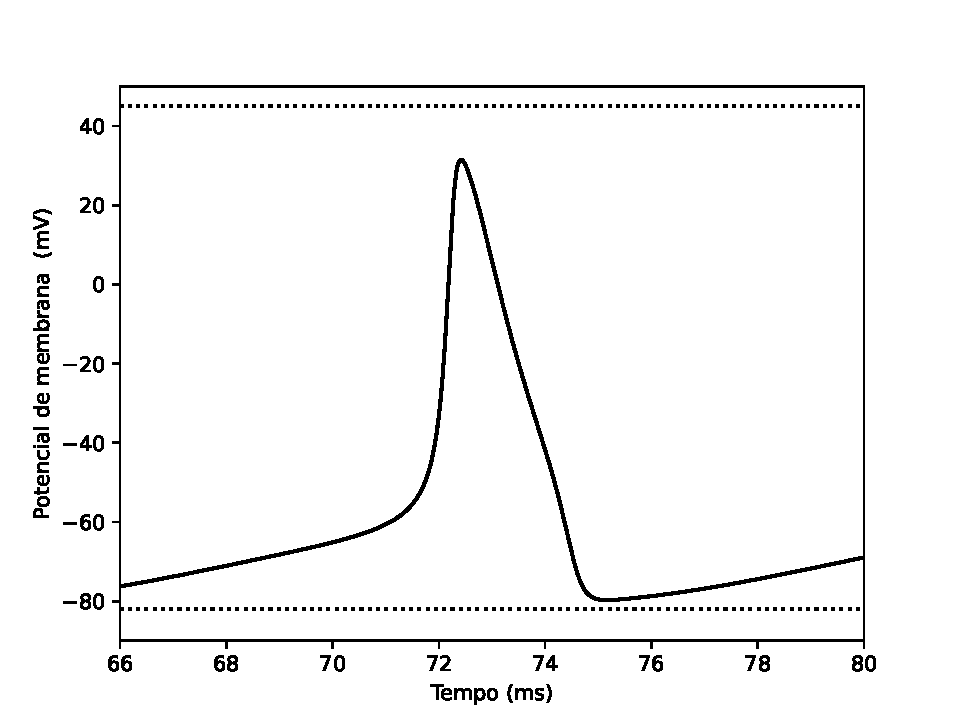
\includegraphics[width=0.7\linewidth]{figs/hh_vm}
\end{figure}
\section{Modelos de taxa de disparo}\label{sec:modelostaxa}

\chapter{Conexões entre neurônios}\label{cap:conexoes}
\section{Introdução}\label{sec:conexoes_intro}

\section{Sinapses}\label{sec:sinapses}
\begin{description}
	\item[Sinapse] Uma conexão entre duas células neuronais. Podem ser de dois tipos:
	\begin{description}
		\item[Sinapses elétricas] se dão a partir de uma junção entre as duas células, por onde íons podem passar, produzindo uma corrente sináptica proporcional à diferença entre os potenciais de membrana das duas células
		\item[Sinapses químicas] são conectadas através de um espaço entre as células, e a interação entre elas se dá pela liberação de neurotransmissores. Podem ser excitatórias, causando despolarização da célula pós-sináptica, ou inibitórias, causando hiperpolarização
	\end{description}
	\item[Neurotransmissor] Um elemento químico que se propaga no espaço entre dois neurônios, fazendo a comunicação entre eles. Os mais comuns associados aos neurônios corticais são o \textbf{glutamato}, que excita a célula pós-sináptica, e o \textbf{ácido $\gamma$-aminobutírico (GABA)}, que a inibe
	\item[Neurônio pré-sináptico] O neurônio que libera o neurotransmissor durante a sinapse após o potencial de ação
	\item[Neurônio pós-sináptico] O neurônio que responde à liberação do neurotransmissor após o potencial de ação do neurônio pré-sináptico
	\item[Vesículas] Compartimentos ao redor da membrana neuronal por onde os neurotransmissores são transportados
\end{description}

\begin{figure}[h!]
	\centering
	\caption{Esquema simplificado de uma sinapse química}
	\label{fig:sinapses}
	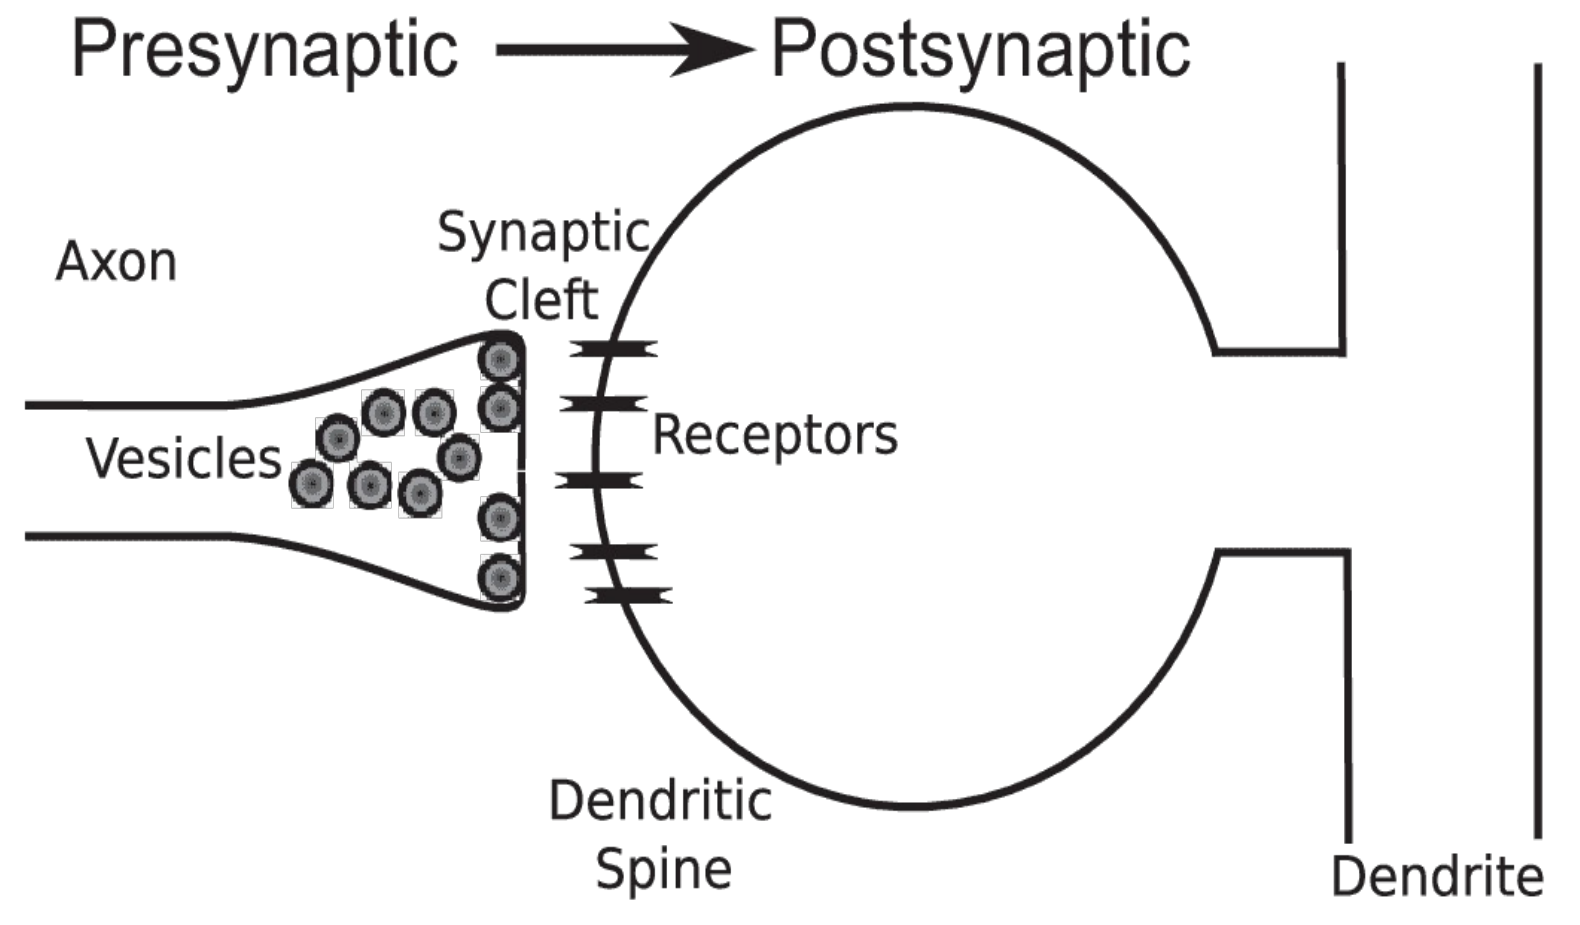
\includegraphics[width=0.7\linewidth]{figs/sinapses}
	\small{Fonte: \cite{miller_introductory_2018}}
\end{figure}


\subsection{Modelagem da transmissão sináptica}
\cite{dayan_theoretical_2001}
O modelo usado é:
$$
\frac{dG_{sin}(t)}{dt}=\frac{-G_{sin}(t)}{\tau_{sin}}
$$
sendo $G_{sin}(t)$ a condutância sináptica e $\tau_{sin}$ a constante de tempo específica para o tipo de sinapse. Além disso, se houver disparo da célula pré-sináptica, ocorre o seguinte mapeamento:
$$
G_{sin}(t)\mapsto G_{sin}(t)+\Delta G
$$
onde $\Delta G$ é o incremento de condutância. Um modelo mais elaborado considera o crescimento e decaimento de condutância usando a equação abaixo:
$$
\Delta G_{sin}(t)=\frac{\Delta G}{K}e^{-(t-t_{disparo})/\tau_{decai}}\Big[1-e^{-(t-t_{disparo})/\tau_{cresce}}\Big]
$$
com $\tau_{cresce}$ a constante de crescimento, $\tau_{decai}$ a constante de decaimento ($\tau_{decai}>\tau_{cresce}$), $t_{disparo}$ o instante do disparo da célula pré-sináptica, e $K$ um fator para garantir que a condutância tenha um valor máximo igual a $\Delta G$, dada por:
$$
K=\Bigg(\frac{\tau_{decai}}{\tau_{cresce}+\tau_{decai}}\Bigg)\Bigg(\frac{\tau_{cresce}}{\tau_{cresce}+\tau_{decai}}\Bigg)^{\tau_{cresce}/\tau_{decai}}
$$

\begin{figure}[h!]
	\centering
	\caption{Condutância sináptica em resposta aos potenciais de ação da célula pré-sináptica}
	\label{fig:respostasinaptica}
	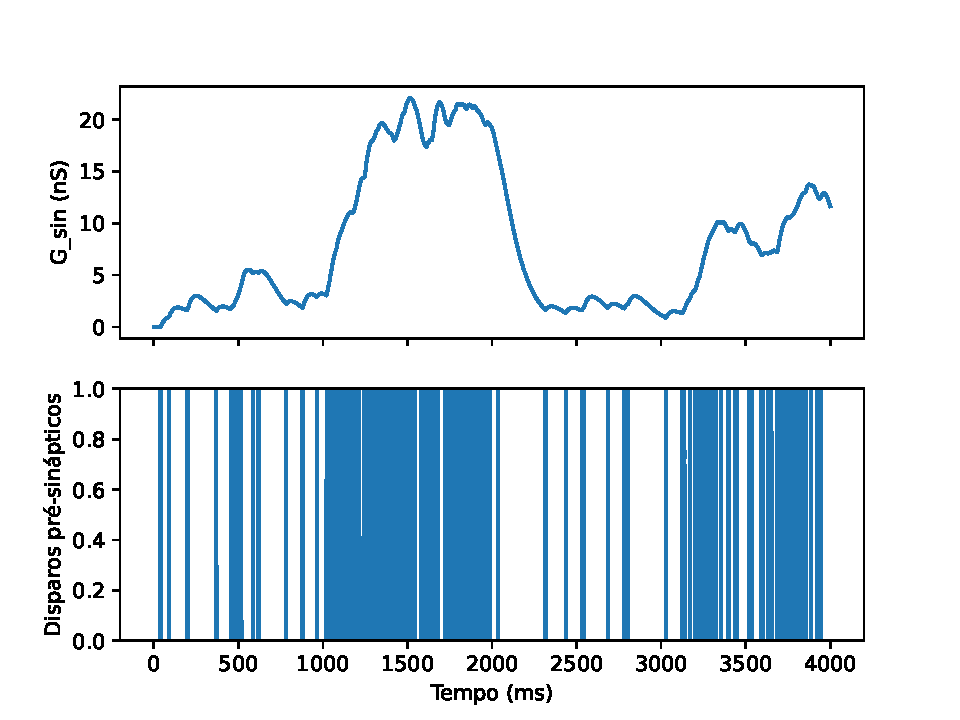
\includegraphics[width=0.8\linewidth]{figs/resposta_sinaptica}
\end{figure}


\section{Sinapses dinâmicas}\label{sec:dinamicas}
\begin{description}
	\item[Sinapse dinâmica] Sinapse cuja força varia em um curto período de tempo
	\item[Depressão de curta duração] Uma redução temporária na força sináptica
	\item[Facilitação de curta duração] Um incremento temporário na força sináptica
\end{description}

A simulação de depressão e facilitação sinápticas é feita alterando-se o valor de $\Delta G$ acima para:
$$
\Delta G=G_{max}p_0FD
$$
com $G_{max}$ o valor máximo de condutância sináptica, $p_0$ a probabilidade de liberação do neurotransmissor, e $F$ e $D$ as variáveis de facilitação e depressão sináptica, atualizadas por:
$$
\frac{dD}{dt}=\frac{1-D}{\tau_D}
$$$$
\frac{dF}{dt}=\frac{1-F}{\tau_F}
$$
e, seguindo cada disparo da célula pré-sináptica:
$$
D\mapsto D-p_0FD\qquad F\mapsto F+f_{fat}(F_{max}-F)
$$
com $F_{max}$ o valor máximo de facilitação e $F_{fat}$ denota o grau de facilitação ($0\leq f_{fat}\leq 1$)

%% falar da bomba de sódio e potassio ao falar do potencial de membrana

\section{Biestabilidade e \textit{feedback} recorrente}\label{sec:biestabilidade}

\subsection{Oscilações e multi-estabilidade}
\begin{description}
	\item[Bi-estabilidade] A capacidade dos neurônios de manter dois estados de atividades mesmo recebendo valores idênticos de entrada
	\item[Oscilações sublimiares] Variações no potencial de membrana insuficientes para a produção de um potencial de ação
	%\item[Quebra do anôdo] Um disparo no potencial de membrana que ocorre logo após uma hiperpolarização
	\item[Ressonância] Uma melhora na resposta de um sistema quando este é estimulado periodicamente com uma frequência particular
\end{description}

\begin{figure}[h!]
	\centering
	\caption{Comportamento variado do modelo de Hodgkin-Huxley}
	\label{fig:hhdinamico}
	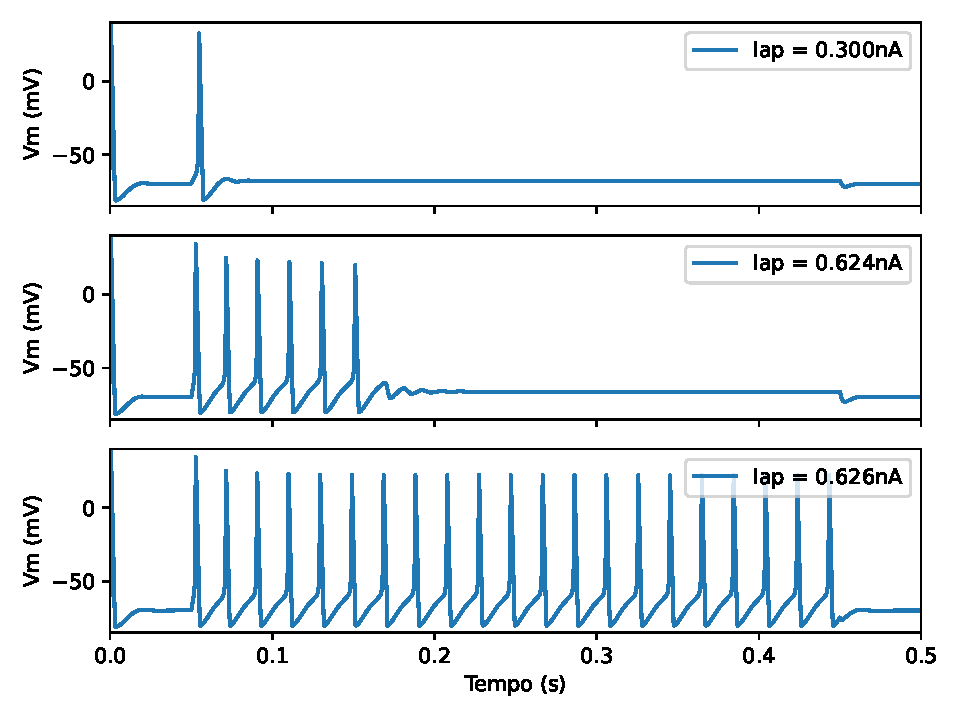
\includegraphics[width=0.7\linewidth]{figs/hh_dinamico}
\end{figure}
% a imagem daqui, das percepções de biestabilidade, está mais para a frente


\begin{description}
	\item[Unidade] Um grupo de neurônios cuja atividade média é simulada
	\item[Feedkback recorrente] Entrada de uma unidade que depende da sua própria atividade
\end{description}

% a imagem ta depois


\subsection{Geradores de padrão central}

\subsection{Circuitos tomadores de decisão}

\section{Caos e criticalidade}\label{sec:caos}
% colocar introdução
% transição de estados
% matemática dos estados

\subsection{Nullclines}
\begin{description}
	% isóclina de inclinação nula
	\item[Fase-plano] \textit{Plots} dos eixos das duas variáveis em um sistema de duas equações diferenciais ordinárias. Mostram os pontos fixos, \textit{nullclines} e trajetórias das variáveis ao longo do tempo
	\item[\textit{Nullcline} (Isóclina de inclinação nula)] Curvas que mostram a dependência de pontos fixos entre as variáveis de um sistema de equações diferenciais ordinárias. Cada equação diferencial gera uma \textit{nullcline}, e as interseções entre elas definem os pontos fixos do sistema
	%\item[Quebra do anôdo] Um disparo no potencial de membrana que ocorre logo após uma hiperpolarização
	\item[Pontos fixos] Pares de valores onde o sistema não se altera (o lado direito da equação diferencial ordinária é igual a 0)
\end{description}

% exemplo lotka-volterra
\begin{figure}[]
	\centering
	\caption{\textit{Nullclines} em sistemas de Lotka-Volterra}
	\label{fig:nullclineslotkavolterra}
	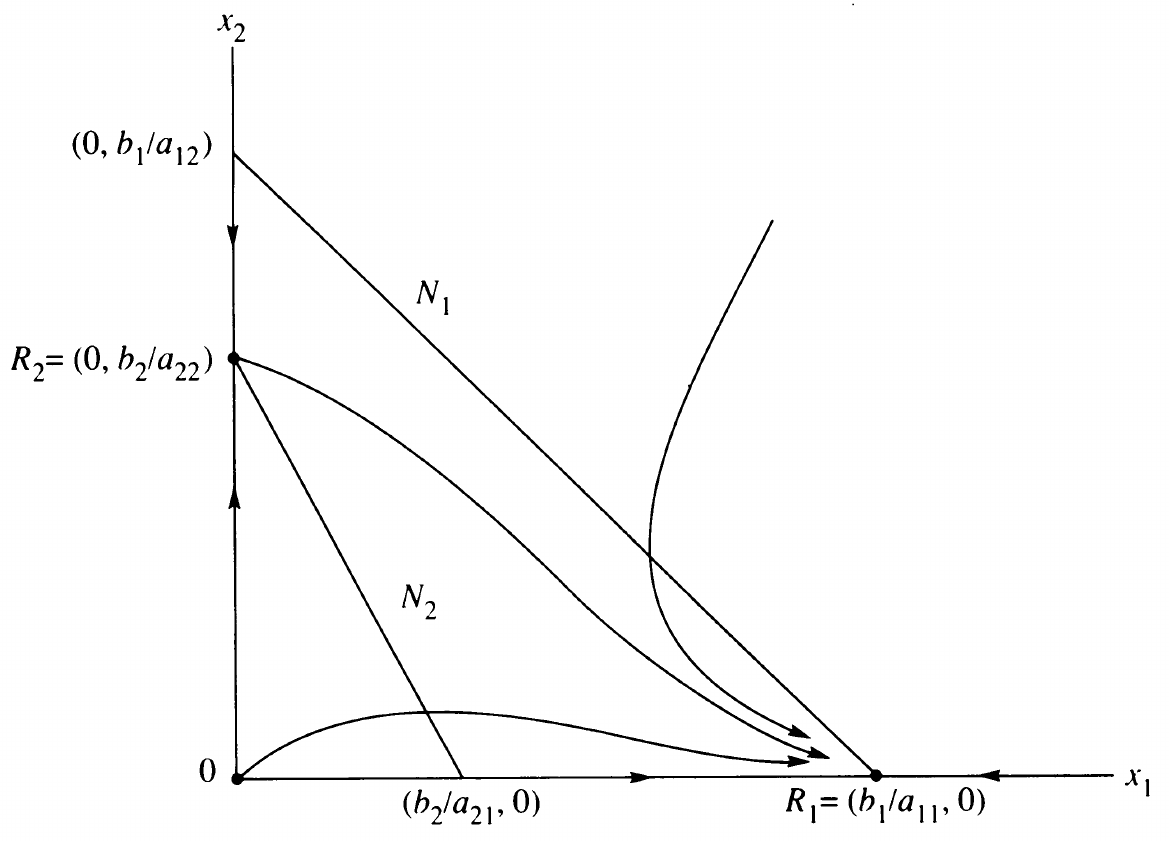
\includegraphics[width=0.7\linewidth]{figs/nullclines_lotka_volterra}\\
	\small{Fonte: \cite{zeeman_extinction_1995}}
\end{figure}

% exemplo fitz-hugh nagumo
\begin{figure}[]
	\centering
	\caption{Plano de fase e estados fisiológicos no modelo FitzHugh-Nagumo}
	\label{fig:fitzhugh}
	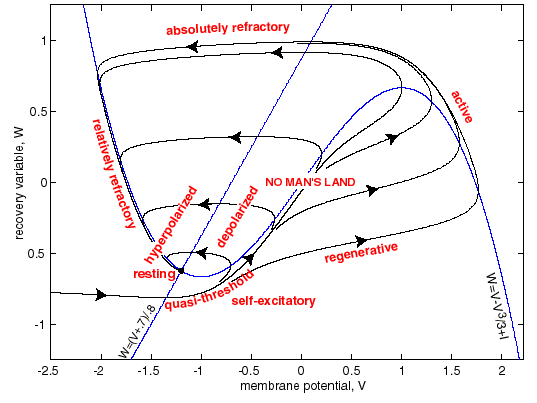
\includegraphics[width=0.7\linewidth]{figs/fitzhugh}\\
	\small{Fonte: Scholarpedia}
\end{figure}

% exemplo izhikevich
% exemplo livro (sistemas bi-estáveis)
\begin{figure}[]
	\centering
	\caption{\textit{Nullclines} mostrando pontos fixos de sistemas bi-estáveis. A linha pontilhada é para $r_2$, e a contínua é para $r_1$. Os pontos fixos, onde as linhas se interceptam, são representados pelos círculos. Os sólidos são pontos estáveis, enquanto os abertos são instáveis.}
	\label{fig:nullcline}
	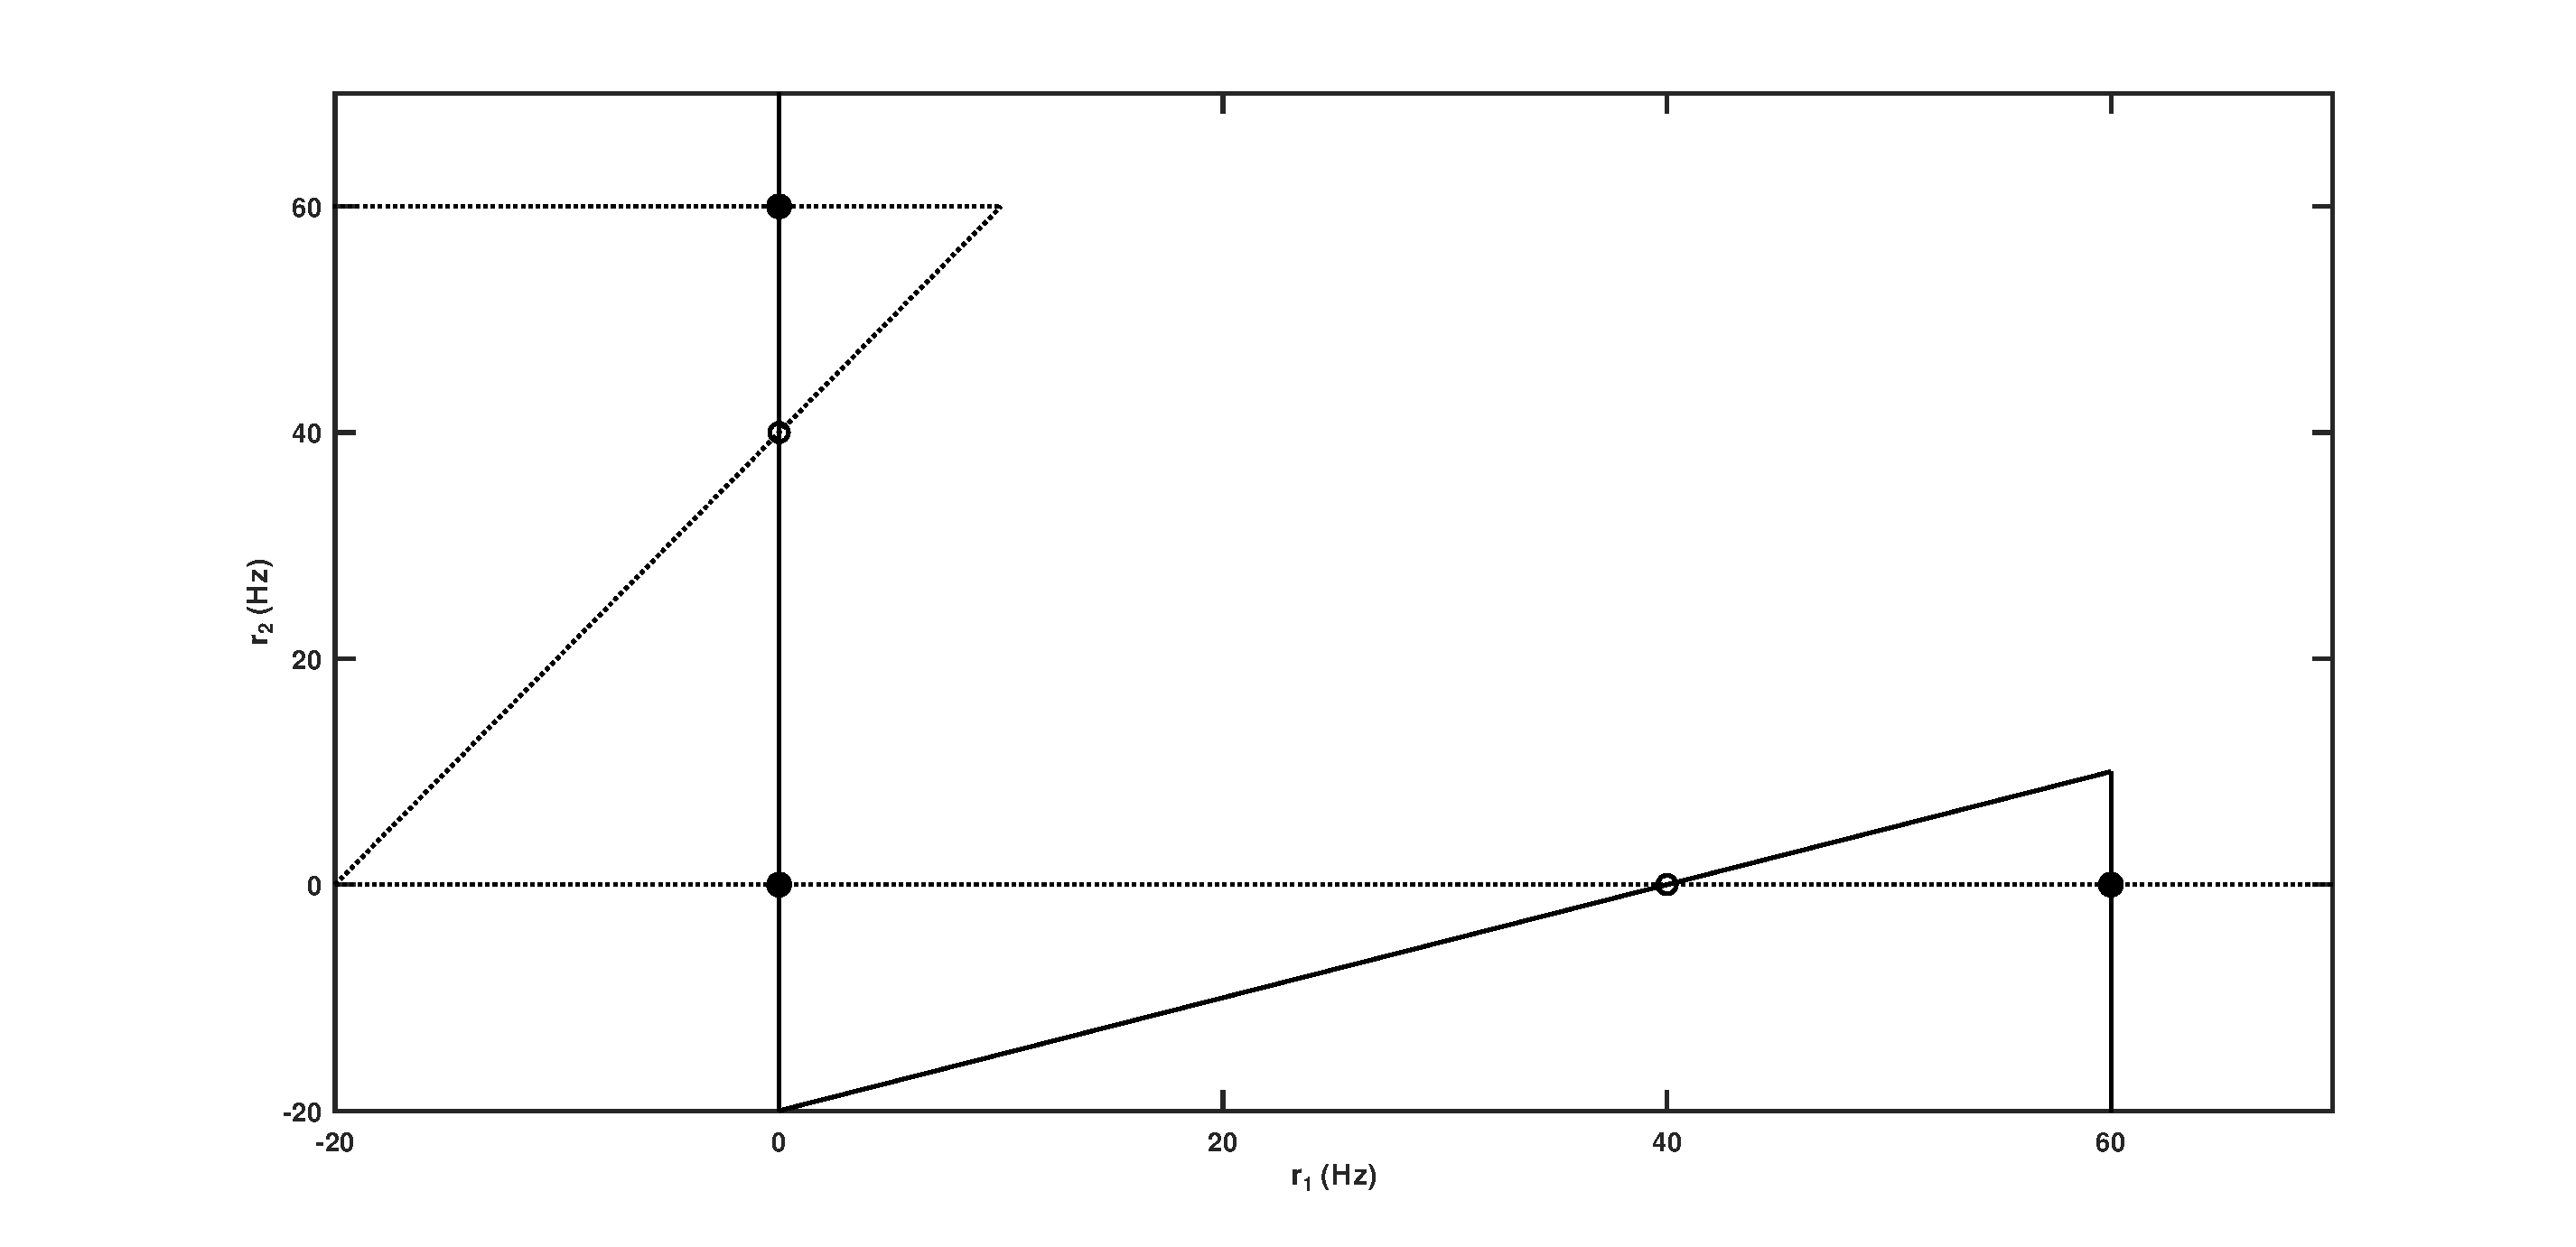
\includegraphics[width=0.9\linewidth]{figs/nullcline}\\
	\small{Fonte: adaptado de \cite{miller_introductory_2018}}
\end{figure}


\subsection{Estados atratores}
\begin{description}
	\item[Intinerância de estados atratores] A mudança de um sistema de um ponto fixo para outro
	\item[Rivalidade perceptual] Estímulos únicos podem ser percebidos de mais de uma maneira, alterando entre cada um dos perceptos (percepções bi-estáveis)
\end{description}

\begin{figure}[]
	\centering
	\caption{Imagens produzindo percepções de bi-estabilidade}
	\label{fig:biestabilidade}
	\begin{subfigure}[h!]{0.3\textwidth}
		\caption{O cubo de Necker pode ser visto com a face frontal em lugares diferentes}
		\label{fig:cubonecker}
		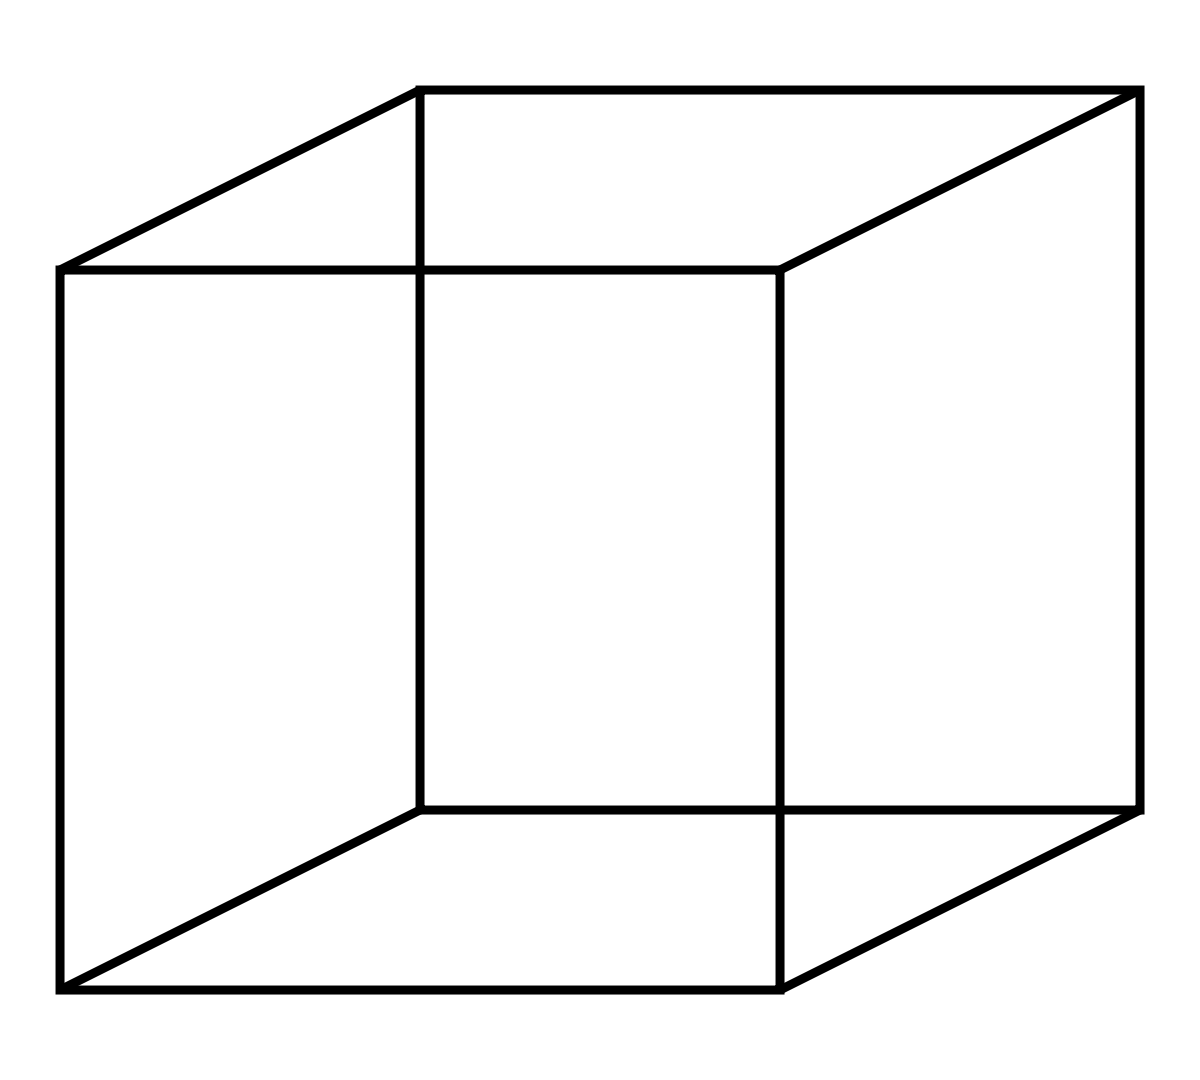
\includegraphics[width=\textwidth]{figs/cubo_necker}
	\end{subfigure}
	\qquad\qquad\qquad
	\begin{subfigure}[h!]{0.3\textwidth}
		\caption{A imagem se assemelha tanto com um cão de frente quanto um homem de costas}
		\label{fig:vasorubin}
		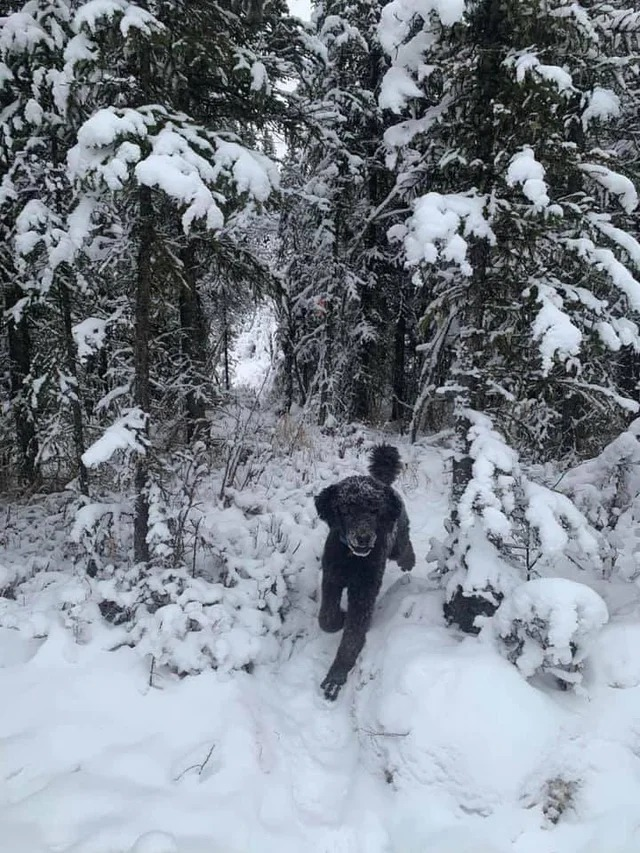
\includegraphics[width=0.8\textwidth]{figs/cao_homem}
	\end{subfigure}
\end{figure}


% indicar o estímulo
\begin{figure}[]
	\centering
	\caption{Unidades de disparo com \textit{feedback} recorrente. A atividade média dos neurônios é simulada, e a saída da unidade também serve como entrada para a mesma. A força da conexão recorrente é excitatória, reforçando a taxa de disparos}
	\label{fig:feedbackrecorrente}
	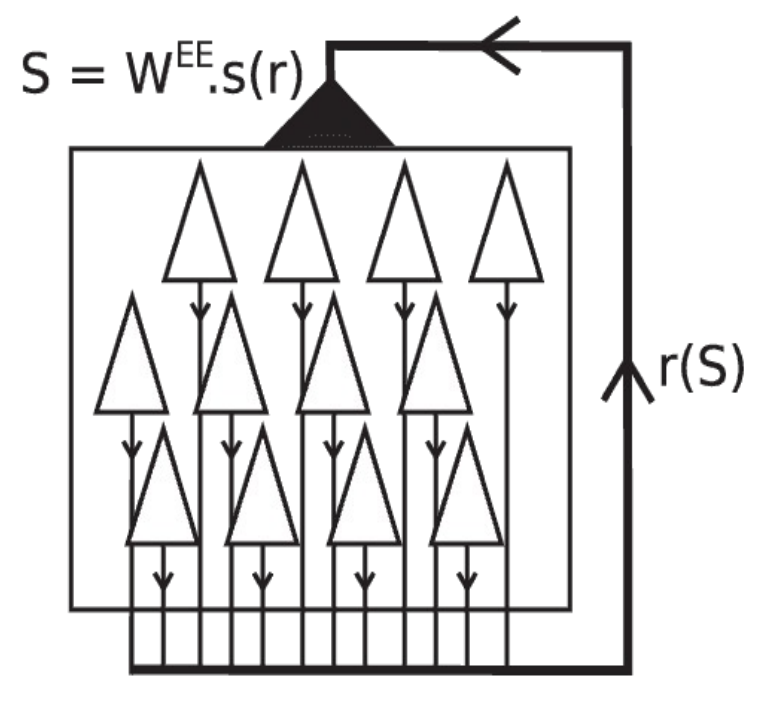
\includegraphics[width=0.45\linewidth]{figs/feedback_recorrente}
\end{figure}
sendo $r(S)$ a taxa média de disparos dos neurônios da unidade, que é função da entrada sináptica total, $S$, da fração de canais sinápticos abertos, $s(r)$, variável entre 0 e 1, multiplicado pela força de feedback, $W^{EE}$, o $EE$ indicando que é um feedback excitatório.
% ligar ambas as figuras
\begin{figure}[]
	\centering
	\caption{Unidade com feedback recorrente que determina a estabilidade de um circuito. A taxa de disparo da unidade é uma função sigmoidal, a linha contínua na direita, e o feedback é representado pela linha tracejada. Na direita, a dinâmica da taxa de disparos em função do tempo, com um pulso de entrada entre 0,5 e 0,55 segundos (a região cinza). O feedback, nesse caso, é médio ($W^{EE}=0.6$), onde taxas baixas e altas de estado são estáveis, causando uma transição entre os estados do sistema}
	\label{fig:biestavel}
	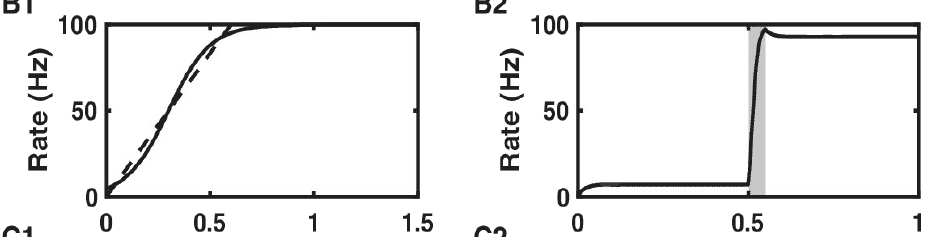
\includegraphics[width=0.7\linewidth]{figs/biestavel}
\end{figure}


\begin{figure}[]
	\centering
	\caption{Unidades de decisão com feedback recorrente e interconexão. As conexões recorrentes são excitatórias, enquanto as interconexões são inibitórias. A presença de ruído, tanto na entrada quanto nas unidades, pode induzir a transições entre estados bi-estáveis}
	\label{fig:unidadesdecisao}
	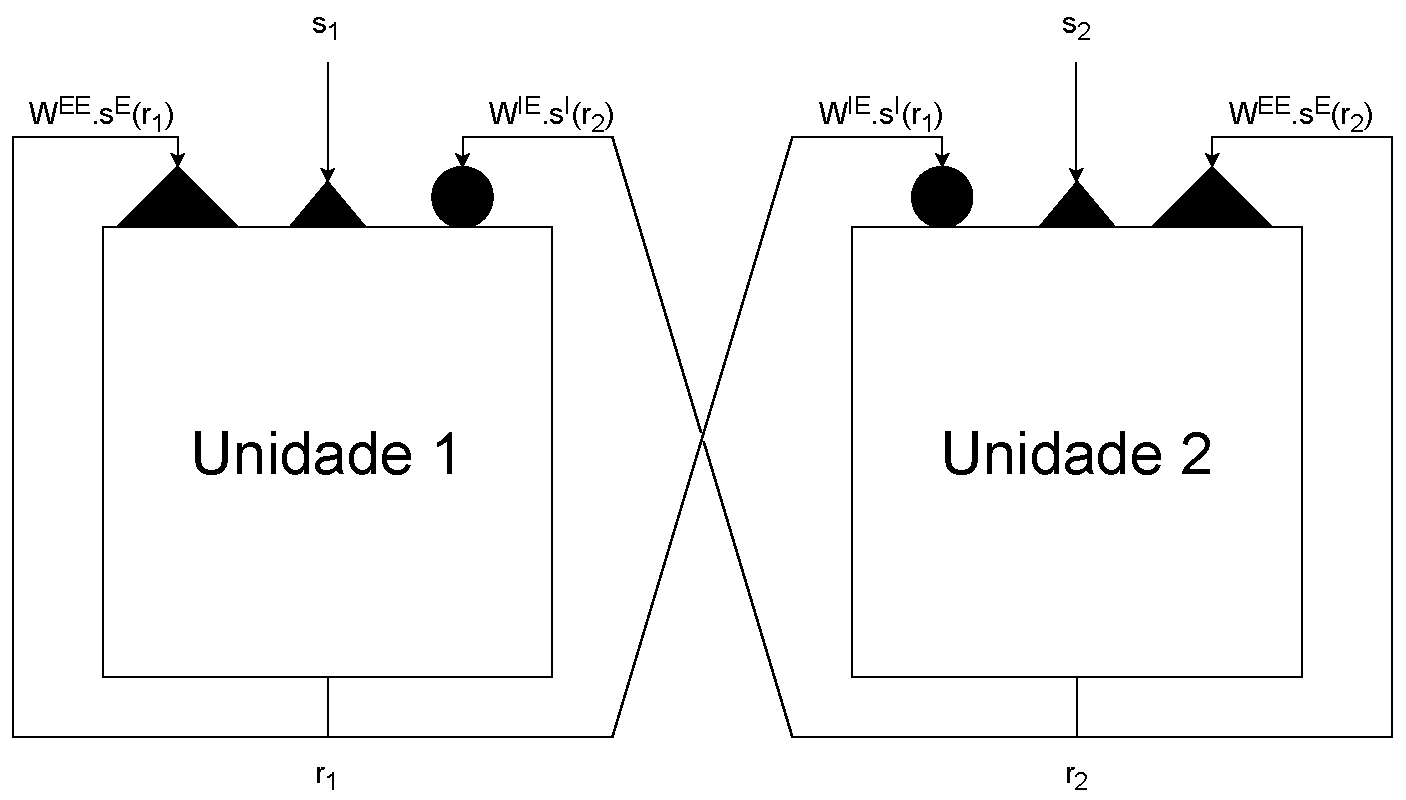
\includegraphics[width=0.7\linewidth]{figs/unidades_decisao}
\end{figure}

\begin{figure}[]
	\centering
	\caption{Transições induzidas por ruído geram intinerância entre dois estados atratores, explicando alternância perceptual. Em (a), três \textit{trials} separados indicando alteração entre os estados, onde a atividade de uma unidade domina sobre a outra. Em (b), a média das atividades ao longo de 10 \textit{trials} (promediação)}
	\label{fig:noiseinducedtransitions}
	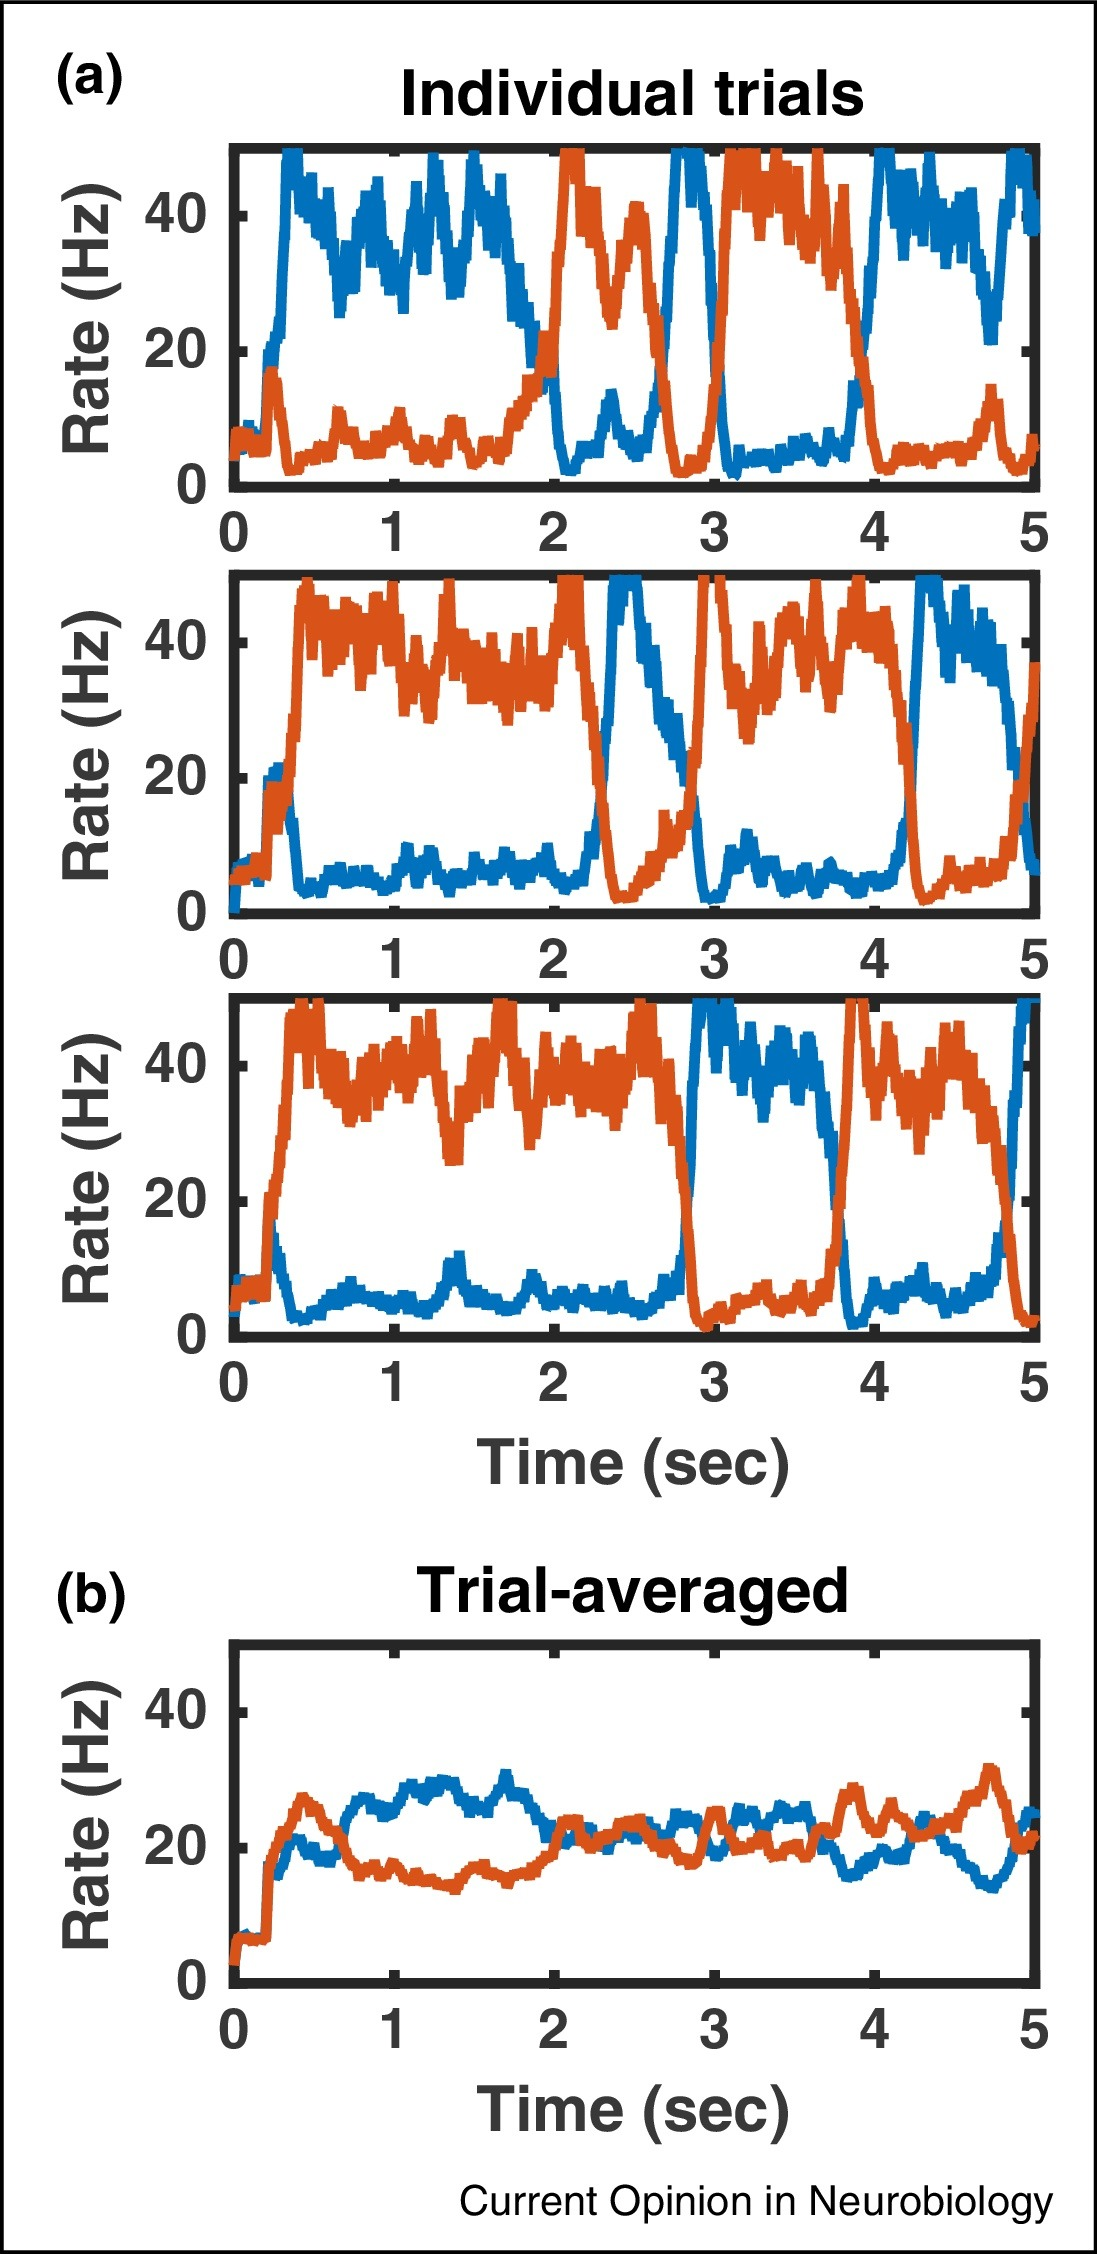
\includegraphics[width=0.35\linewidth]{figs/noise_induced_transitions}
\end{figure}


\subsubsection{Múltiplos atratores}
\begin{itemize}
	\item Alterações para mais de dois estados perceptuais
	\item Podem ser representados usando modelos ocultos de Markov (HMM, \textit{Hidden Markov Models})
	\item Na Figura~\ref{fig:hmm}, em (b), são mostrados os estados discretos que o HMM pode assumir nesse caso (círculos coloridos), com as matrizes de probabilidades de transição entre estados por unidade (a espessura das setas).
	\item Cada estado é definido pela probabilidade de emissão de um padrão particular em um intervalo de tempo (histogramas dentro dos círculos)
\end{itemize}

\begin{figure}[]
	\centering
	\caption{Modelos ocultos de Markov. Em (a), os conjuntos de trens de disparo de potenciais de ação. Em (b), os estados discretos que o HMM assume. Em (c), as probabilidades a posteori para cada estado}
	\label{fig:hmm}
	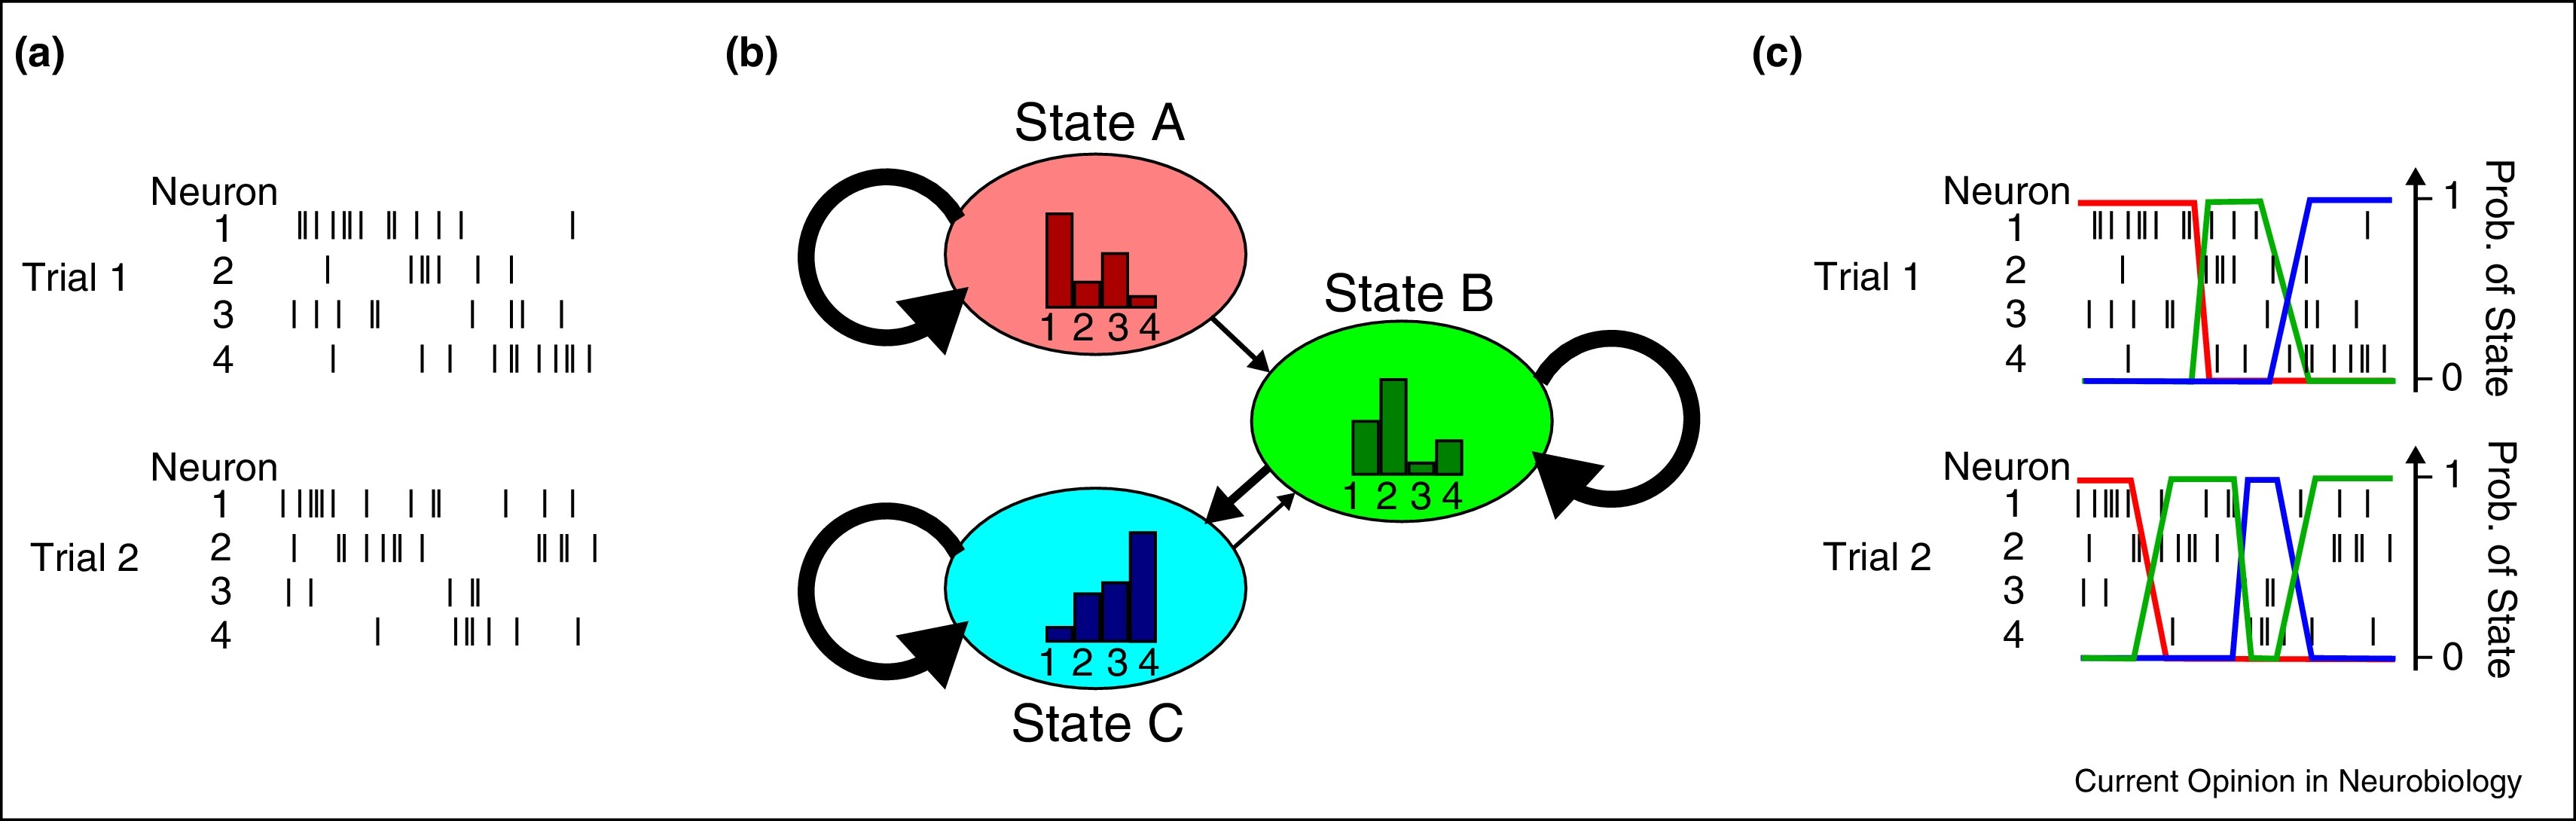
\includegraphics[width=0.8\linewidth]{figs/hmm}
\end{figure}


\subsection{Caos}
\begin{itemize}
	\item A \textbf{teoria do caos} é um ramo da matemática que lida com sistemas dinâmicos não lineares, ou seja, a interação dos componentes do sistema não é somente a adição desses componentes individualmente, devido a existência de efeitos multiplicativos ou de \textit{feedback}
	\item Sistemas caóticos podem ter poucas partes e seguirem regras bem simples, porém possuem uma sensibilidade bem grande às condições iniciais, onde o impacto de um pequeno efeito pode crescer exponencialmente ao longo do tempo
	\item A dinâmica não-linear de sistemas com caos facilita a habilidade de adaptação presente em sistemas neuronais, causando transições de um padrão de comportamento para outro quando o ambiente é alterado e, consequentemente, criando uma rica variedade de padrões
	\item Sistemas operam na \textbf{beira do caos} quando, para um mesmo conjunto de parâmetros, se ajustados em uma direção tornam o sistema caótico, enquanto que se ajustados em outra direção fazem com que o sistema apresente estados estáveis
	\item O conjunto de parâmetros, na condição de beira do caos, pode ser chamado de crítico, com o sistema podendo exibir \textbf{criticalidade}, uma propriedade dos sistemas onde uma pequena alteração do sistema em um local pode tanto ter um efeito local quanto se propagar e alterar o sistema como um todo
	\item Acredita-se que sistemas em criticalidade possuem melhores capacidades de processamento de informação e otimização de memória, inspirando a hipótese da criticalidade, proposição onde o cérebro opera em um estado crítico, devido às capacidades de computação ótimas associadas precisarem ser evolutivamente selecionadas para isso
	\item A ideia geral de sistemas se auto migrarem para estados críticos através de processos descentralizados é conhecido como \textbf{criticalidade auto-organizável} (SOC, \textit{self-organized criticality})
	\item Uma cascata de disparos de atividade neuronal que ultrapassa um limiar em intervalos de tempo seguidos é chamado de \textbf{avalanche} (Fig.~\ref*{fig:sandpile})
	\item Exemplos de sistemas que podem exibir comportamento caótico incluem o modelo de neurônio de Izhikevich (já visto) e a equação do mapa logístico (tutorial), dada por $x_{t+1}=rx_t(1-x_t)$, e que representa um modelo discreto de crescimento populacional, sendo $x_t$ a taxa de população no tempo $t$ e $r$ a taxa de crescimento
\end{itemize}

\begin{figure}[]
	\centering
	\caption{Modelo de pilha de areia}
	\label{fig:sandpile}
	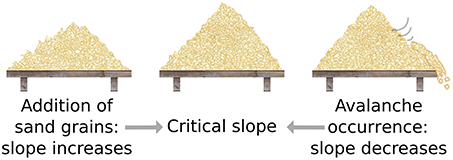
\includegraphics[width=0.7\linewidth]{figs/sandpile}
\end{figure}


%\subsection{Coeficiente de Lypunov}

%\subsection{Avalanches}

\chapter{Plasticidade de curta duração}\label{cap:plasticidade}
\section{Introdução}\label{sec:plasticidade_intro}

\chapter{Aprendizado e plasticidade de longa duração}\label{cap:aprendizado}
\section{Introdução}\label{sec:aprendizado_intro}

\chapter{Inteligência artificial}\label{cap:ia}
\section{Introdução}\label{sec:ia_intro}
Redes neurais artificiais são alguns tipos de modelos computacionais do cérebro. Tratam-se da interconexão entre unidades de processamento, geralmente neurônios artificiais. Os tipos de rede variam com o tipo de aprendizado e a arquitetura. Alguns tipos de aprendizado são os seguintes:

\begin{description}
	\item[Aprendizado supervisionado] Mapeia as entradas e saídas baseado em pares de entrada-saída de exemplo, que são rotulados (uma entrada tem a sua saída definida)
	\item[Aprendizado não-supervisionado] Aprende padrões de dados não rotulados
\end{description}

Existem diversos tipos de redes neurais artificiais, e algumas delas estão mostradas na Figura~\ref{fig:neuraltypes}.

\begin{figure}[htb!]
	\centering
	\caption{Alguns tipos de redes neurais}
	\label{fig:neuraltypes}
	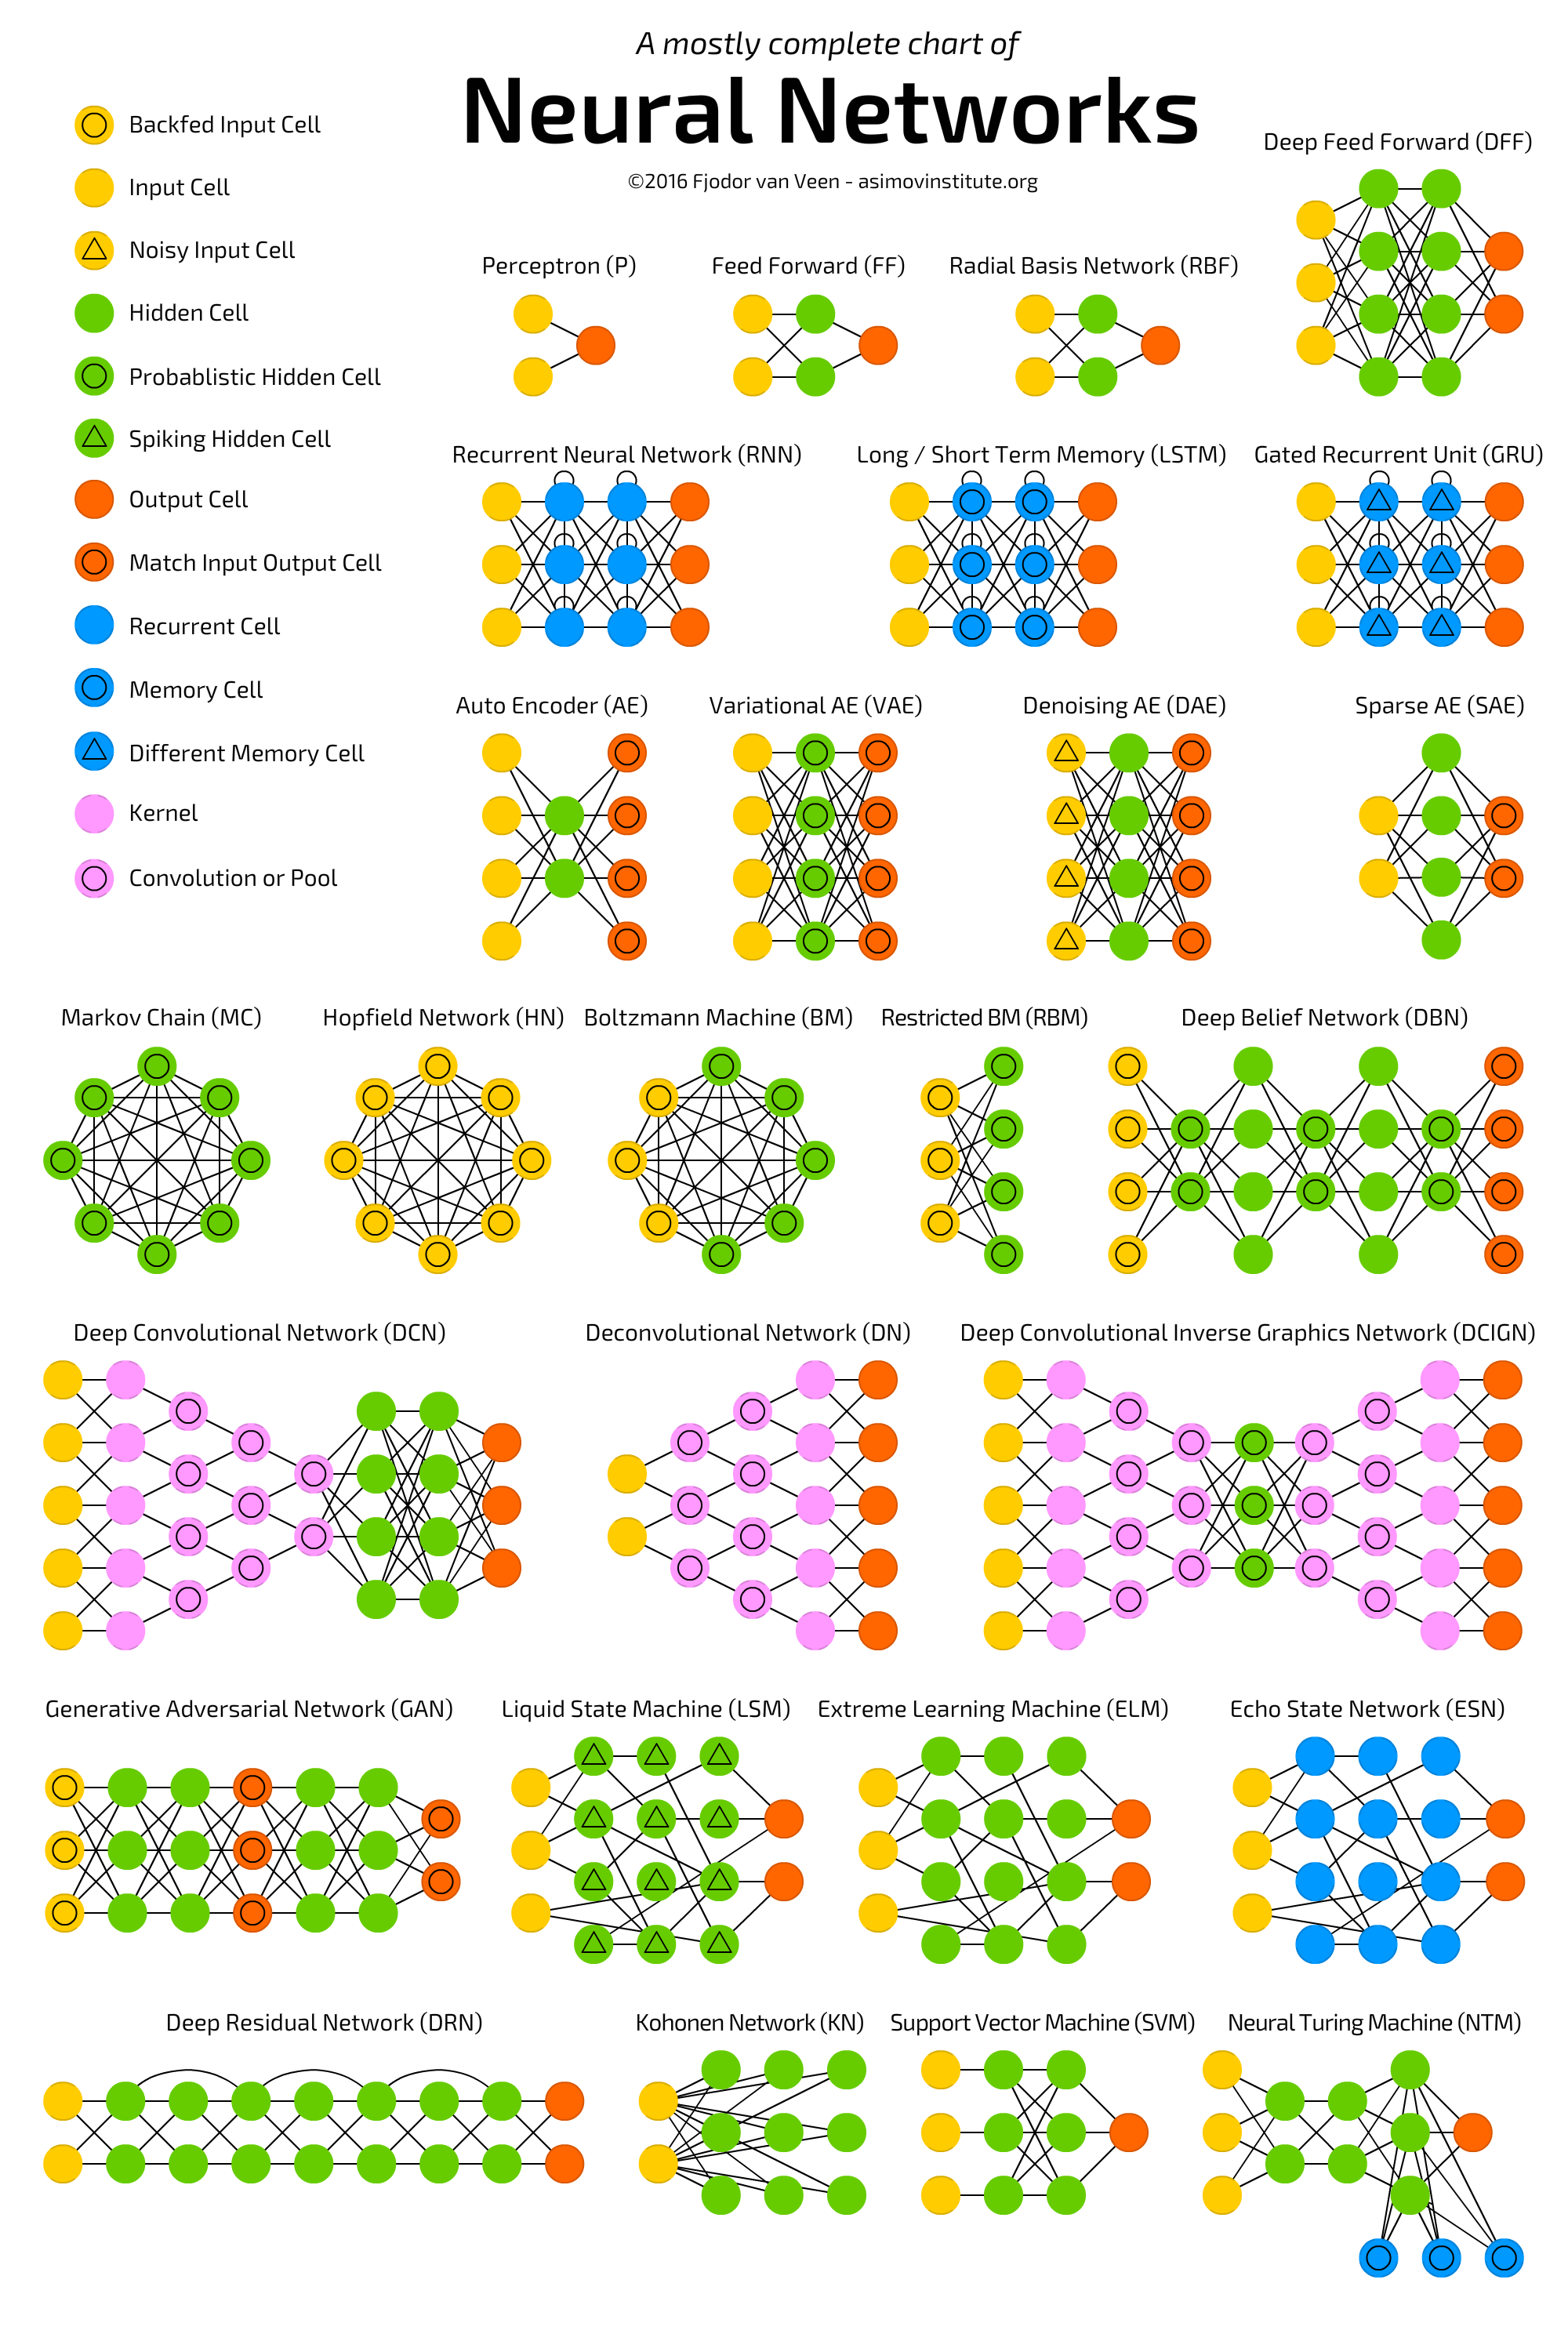
\includegraphics[width=0.34\linewidth]{figs/neural_types}
\end{figure}

Alguns desses tipos são descritos abaixo:

\begin{description}
	\item[Perceptron] Primeiro modelo de neurônio artificial. É um classificador binário com uma função de ativação do tipo degrau
	\item[Perceptron de múltiplas camadas (MLP, \textit{Multilayer perceptron})] Combinação de vários neurônios do tipo perceptron em pelo menos três camadas: uma de entrada, uma oculta e uma de saída (Figura~\ref*{fig:modelosmlp}). Utiliza a técnica de aprendizado chamada \textit{backpropagation}, onde as atualizações dos pesos é feita da camada de saída em direção à de entrada. A grande maioria das redes neurais artificiais é derivada da MLP
	\item[Redes neurais profundas] Rede neural com uma grande quantidade de camadas ocultas. Alguns subtipos incluem as \textbf{Redes neurais recorrentes}, em que os dados fluem em qualquer direção, permitindo os neurônios enviarem \textit{feedback} uns para os outros (a rede Hopfield é uma delas), e as \textbf{Redes neurais convolucionais}, que aplicam uma operação de convolução e são bastante usadas em tarefas de visão computacional
	\item[Redes neurais de disparo (SNN, \textit{Spiking Neural Networks})] Redes onde a unidade computacional é um neurônio de disparo
\end{description}

\begin{figure}[htb!]
	\centering
	\caption{Modelos básicos de neurônios e redes neurais. Em (a), o perceptron com uma função de ativação do tipo degrau; em (b), o perceptron com uma função de ativação sigmoide; em (c), uma rede neural com uma camada oculta}
	\label{fig:modelosmlp}
	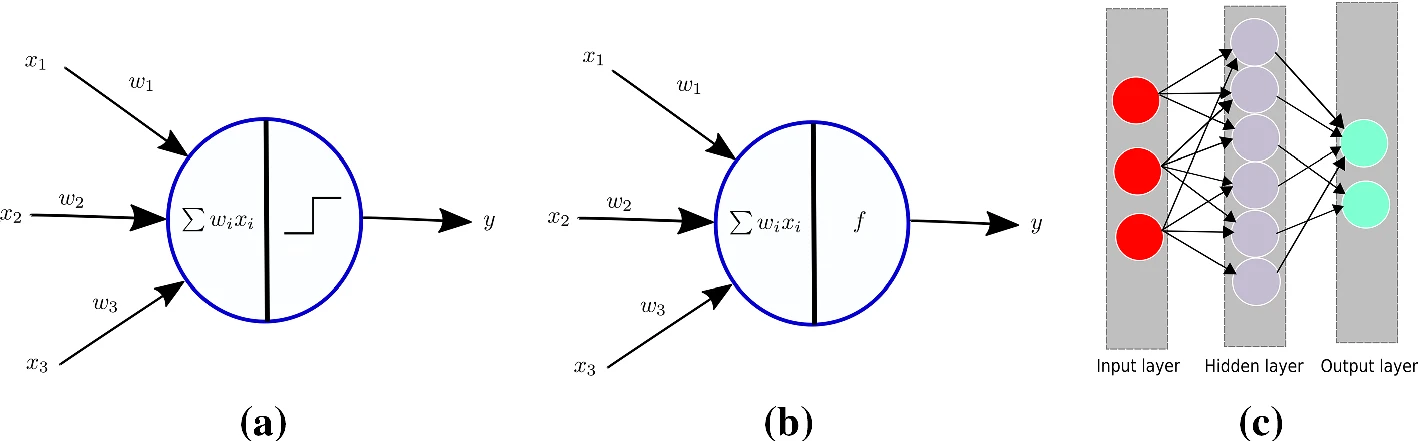
\includegraphics[width=0.9\linewidth]{figs/modelos_mlp}
\end{figure}


\section{Redes neurais}\label{sec:redesneurais}
\subsection{Redes \textit{feed-foward}}
% backprop/grad desc

\subsection{Redes recorrentes}
% lstm

\section{Redes neuromórficas}\label{sec:redesneuromorficas}
% estado da arte
% hardware neuromórfico (von-neumann vs neuromorfico)

\begin{itemize}
	\item Redes neurais de disparo usam neurônios de disparo como unidades de computação, como os modelos \textit{Leaky integrate-and-fire} (LIF) e o modelo de Izhikevich
	\item As unidades de computação são conectadas entre si e interagem através das sinapses (Figura~\ref{fig:sinapse})
\end{itemize}

\begin{figure}[htb!]
	\centering
	\caption{Neurônios pré (verde) e pós (roxo) sinápticos conectados através de uma sinapse. Os neurotransmissores (círculos vermelhos) são liberados do axônio pré-sinaptico para o dendrito pós-saptico, gerando potenciais pós-sinapticos que podem ser excitatórios (EPSP) ou inibitórios (IPSP). No neurônios pós-sinaptico os potenciais de todos os dendritos são somados e, dependendo do valor total, um potencial de ação (AP) pode ser gerado}
	\label{fig:sinapse}
	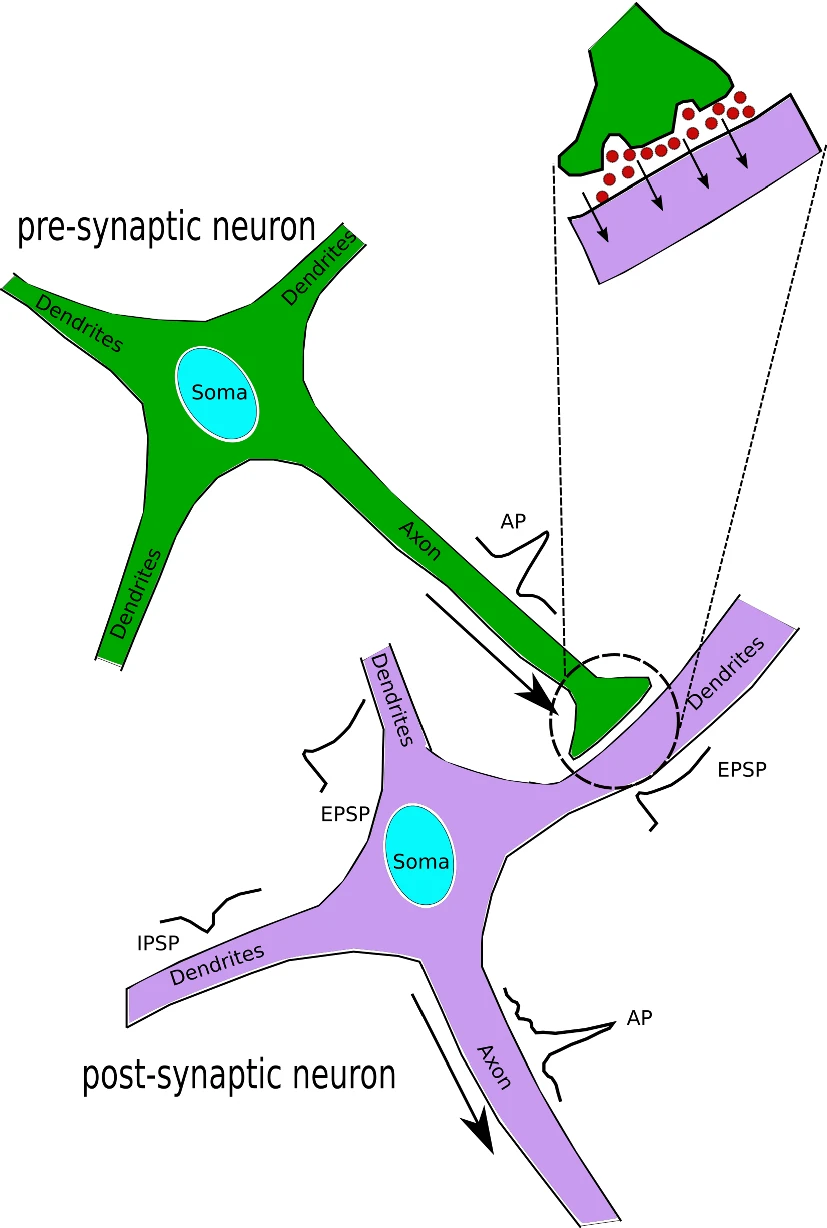
\includegraphics[width=0.3\linewidth]{figs/sinapse}
\end{figure}

\subsection{Processamento de informação}
\begin{itemize}
	\item A informação recebida pelas redes precisa ser codificada, e dois métodos para isso são:
	\begin{description}
		\item[Codificação de taxa] A taxa de disparo dos neurônios é usada. A taxa pode ser calculada como a média temporal (quantidade de disparos por intervalo de tempo), média de disparos em \textit{trials} diferentes, dentre outras maneiras
		\item[Codificação de tempo de disparo] O instante exato de ocorrência de disparos individuais é usado. Dentre os tipos de codificação nesse caso incluem-se o tempo do primeiro disparo (o tempo entre o início do estímulo e a ocorrência do primeiro disparo), a codificação de ordem (a ordem em que os neurônios disparam é o código), a codificação de latência (a diferença de tempo entre os disparos), dentre outras
	\end{description}
	\item Os critérios para seleção do método de codificação variam por diferentes aspectos, como a \textbf{minimização da perda de informação após a decodificação} e o \textbf{aumento da acurácia de previsão/classificação}
\end{itemize}

\subsection{Aprendizado das redes de disparo}
\begin{itemize}
	\item Para cada tipo de codificação citada acima, um método de aprendizado é empregado, que são:
	\begin{description}
		\item[Aprendizado baseado em taxa] Uma variação do método \textit{backpropagation} é usada aqui, relacionando as ativações das unidades das redes neurais com as taxas de disparo
		\item[Aprendizado baseado em disparo] Utiliza a plasticidade dependente de tempo de disparo (STDP, \textit{spike-timing dependent plasticity}),onde os pesos das conexões sinapticas são proporcionais ao grau de relação entre os tempos de disparo pré e pós-sinapticos (Figura~\ref{fig:stdp})
	\end{description}
\end{itemize}

\begin{figure}[htb!]
	\centering
	\caption{Conceito da STDP}
	\label{fig:stdp}
	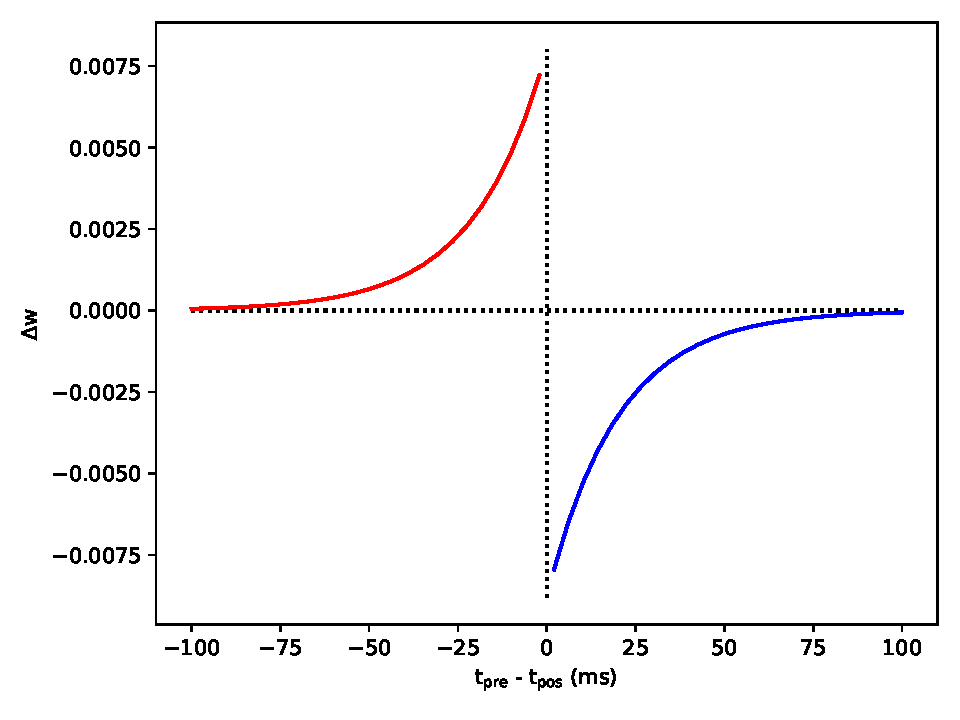
\includegraphics[width=0.7\linewidth]{figs/stdp}
\end{figure}



% pensar onde colocar os simuladores
% \section{Simuladores neuronais}\label{sec:simuladores}

%\chapter{Análise de sinais de eletroencefalograma}\label{cap:eeg}

% ----------------------------------------------------------
% Considerações Finais
% ----------------------------------------------------------
\chapter{Considerações finais}\label{cap:conclusoes}
Este trabalho apresentou uma série de conteúdos para a execução de um curso introdutório de neurociência computacional, voltado para diversos públicos, servindo como um guia de execução. Baseado em algumas execuções do curso, uma possível sequência didática para o mesmo é mostrada na Tabela~\ref{tab:sequencia_didatica}.
\begin{table}[tb]
	\IBGEtab{
		\caption{Proposta de sequência didática}
		\label{tab:sequencia_didatica}
	}{
	\begin{tabular}{|c|c|p{8cm}|}
	\hline
	Número da aula & Tema & Conteúdo \\
	\hline
	1 & Apresentação da disciplina & Apresentação do estado da arte \\
	\hline
	2-4 & Introdução & Neurobiologia; equações diferenciais; introdução ao Python \\
	\hline
	5-9 & Modelos de neurônio de disparo & Modelos LIF, ELIF, AELIF, Izhikevich, Hodgkin-Huxley \\
	\hline
	10-17 & Conexões entre neurônios & Sinapses; Sinapses dinâmicas; Multi-estabilidade; Modelos de Wilson-Cowan; Aprendizado \\
	\hline
	18-21 & Inteligência artificial & Redes neurai; Redes neuromórficas \\
	\hline
	22-24 & Conclusão & Apresentações/entregas de trabalhos; Avaliação da disciplina \\
	\hline
	\end{tabular}
}{
\fonte{o autor (\the\year)}
}
\end{table}
Também baseado em execuções do curso, foi elaborada a proposta de atividades avaliativas, referentes a cada capítulo apresentado, como segue:
\begin{alineas}
	\item Introdução: questões simples de neurobiologia, equações diferenciais e implementações de códigos em Python;
	\item modelos: alterações de parâmetros nos modelos LIF, ELIF e/ou AELIF;
	\item conexões: implementação de circuitos de multi-estabilidade com o modelo de Wilson-Cowan;
	\item tarefa final: implementação de codificação para a rede de disparo.
\end{alineas}

A proposta de execução do curso é utilizando o Google Colaboratory (Colab), que fornece um ambiente de programação em Python gratuito, incluindo recursos de \textit{hardware} robustos para aplicações de aprendizado de máquina.
%TODO: citação bisong google colaboratory
Como exibido na Figura~\ref{fig:colab}, o Colab é executado a partir de um \textit{Notebook}, que facilita a execução e reprodução de códigos e conteúdos em conjunto.
%TODO: citação interactive
Todos os códigos-fonte utilizados durante o curso, incluindo os que geram algumas das imagens deste texto, estão disponíveis em repositório online\footnote{\url{https://gitlab.com/weversonvn/intro_neurocomp}}, de maneira gratuita e com uma licença permissiva livre para uso.
\begin{figure}[tb]
	\centering
	\caption[Ambiente do Google Colaboratory com o conteúdo de neurônios de disparo]{Ambiente do Google Colaboratory com o conteúdo de neurônios de disparo}
	\label{fig:colab}
	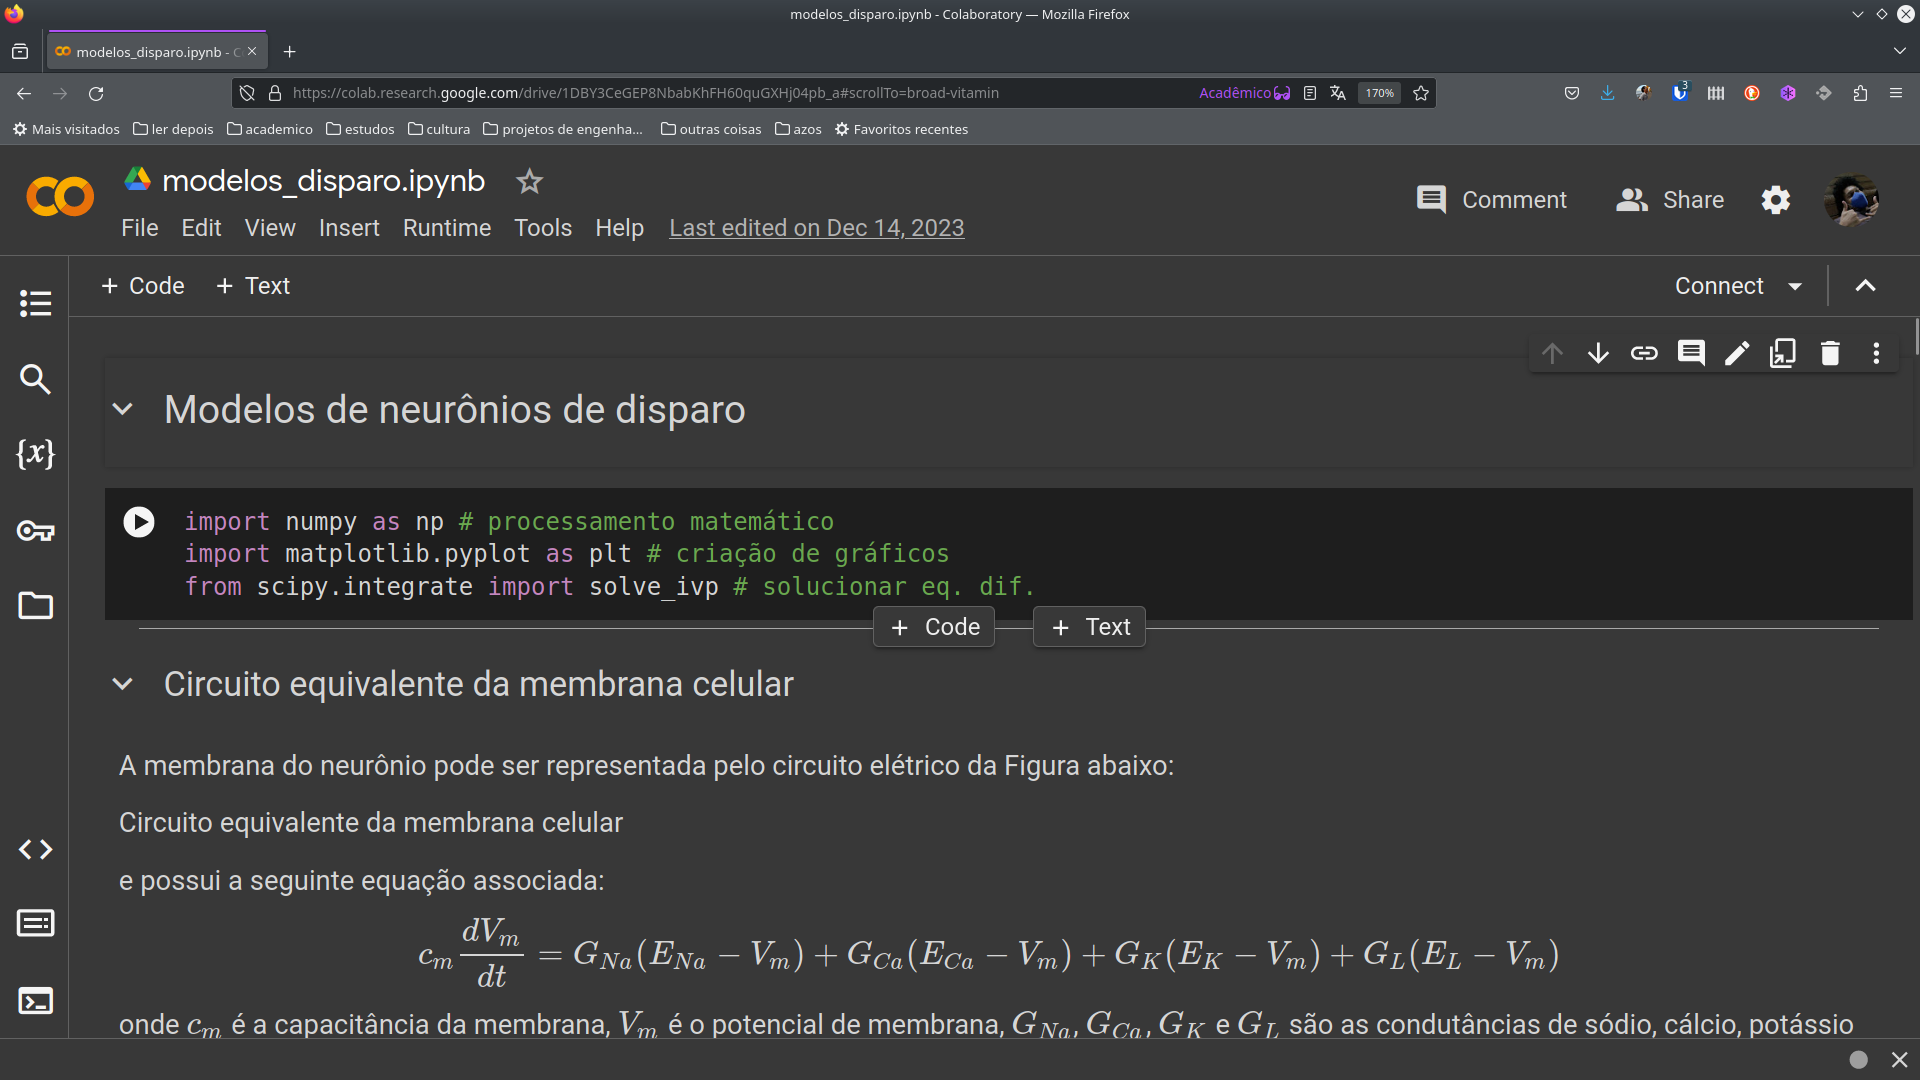
\includegraphics[width=0.7\linewidth]{figs/colab}
	\legend{Fonte: o autor (\the\year)}
\end{figure}

Possíveis melhorias para o curso começam pelo refinamento dos conteúdos já existentes, baseado nas considerações que venham a ser obtidas por eventuais alunos que o façam, como a alteração da ordem dos conteúdos, maior detalhamento de algum tópico específico, diminuição de outros. Além disso, um material voltado para exercícios pode ser bastante útil, tanto dos conteúdos teóricos quanto dos práticos, com destaque para tarefas em Python voltadas para cursos onde o público alvo não tem grande familiaridade com a linguagem ou com programação.

Como conteúdos novos pode-se incluir a simulação de modelos multi-compartimento, com destaque para a estimulação elétrica axonal, para estudar a propagação do potencial de ação ao longo do axônio.
%TODO: citação rattay a model
Outra possibilidade é a análise de sinais de eletroencefalograma (EEG), que são respostas elétricas obtidas das atividades cerebrais, podendo ser utilizadas para associações com comorbidades, como depressão e ansiedade.
%TODO: cavanagh multiple
Por fim, a apresentação de pacotes do Python voltados para análises semelhantes às apresentadas no curso pode ser incluído, uma vez que o uso destes potencialmente se torna mais simplificado com o entendimento obtido a partir do conteúdo deste trabalho.

% ---

% ----------------------------------------------------------
% ELEMENTOS PÓS-TEXTUAIS
% ----------------------------------------------------------
\postextual
% ----------------------------------------------------------

% ----------------------------------------------------------
% Referências bibliográficas (obrigatório - NBR 6023)
% ----------------------------------------------------------
% Os elementos essenciais são: autor(es), título, edição, local, editora e data de publicação
%  Quando se tratar de obras consultadas online,  também  são  essenciais  as  informações  sobre  o  endereço  eletrônico, apresentado  entre  os  sinais  <  >,  precedido  da  expressão  Disponível  em:  e  a  data  de  acesso  ao  documento,  precedida  da expressão Acesso em:, opcionalmente acrescida dos dados referentes a hora, minutos e segundos

% o template já faz no formato adequado
% eu fiz um arquivo .bib separado que é importado aqui
\bibliography{neurocomp}
% ---

% antes do apêndices um item opcional é o glossário
% se incluído é em ordem alfabética

% ----------------------------------------------------------
% Apêndices (opcional)
% ----------------------------------------------------------

% ---
% Inicia os apêndices
% ---
%\begin{apendicesenv}
	
	% Imprime uma página indicando o início dos apêndices
	% a norma não diz para criar essa página
%	\partapendices

% usar um include com \chapter para cada apêndice
	
%\end{apendicesenv}
% ---

% ----------------------------------------------------------
% Anexos (opcional)
% ----------------------------------------------------------

% ---
% Inicia os anexos
% ---
%\begin{anexosenv}
	
	% Imprime uma página indicando o início dos anexos
	% novamente a norma não diz para criar essa página
%	\partanexos

% novamente usar um include com \chapter para cada anexo
% ou usar \includepdf caso seja documento externo (o mais provável no caso de anexo)
	
%\end{anexosenv}

% o último item opcional é o índice
% se incluído é conforme a NBR 6034

\end{document}
